\documentclass[a4paper, 11pt]{report}

% LEVEL 5 UNIVERSITY NOTES PREAMBLE
% THOMAS BOXALL <thomas@thomasboxall.net>
% 12 September 2023
%%%%%%%%%%%%%%%%%%%%%%%%%%%%%%%%%%%%%%%%%

% this preamble gets include in all university note documents. It contains custom stylling and useful features to speed up note taking.

%%%%%%%%%%%%%%%%%%%%%%%%
% Basic Document Setup %
%%%%%%%%%%%%%%%%%%%%%%%%

\usepackage{geometry}
\geometry{
a4paper,
total={170mm,257mm},
left=20mm,
top=20mm,
marginparsep=0mm,
}
\setlength\parindent{0pt} % get rid of the stupid indent

% add in capabilities for small notes in the left margin
\reversemarginpar
\newcommand{\marginnote}[1]{%
\marginpar{\footnotesize\texttt{#1}}
}

% set toc depth to only show chapters
\setcounter{tocdepth}{0}

% use section numbering for everything up too and including subsubsection
\setcounter{secnumdepth}{3}

% BASIC PACKAGES
\usepackage[dvipsnames]{xcolor}
\usepackage{graphicx}
\usepackage{fontawesome}
\usepackage[colorlinks=true, linkcolor=myBlue]{hyperref}
\usepackage{lastpage}
\usepackage{datetime2} % changes \today format to be yyyy-mm-dd
\usepackage{enumitem}
\usepackage{amsmath}
\usepackage{amssymb}

\usepackage{smartdiagram} % used for fancy diagrams.
\usepackage{pgf, tikz}
\usepackage{pgfplots}
\pgfplotsset{compat=1.11}
\usetikzlibrary{arrows, automata, arrows.meta, bending, positioning, trees, patterns, calc}

% CUSTOM COLOURS
\definecolor{myGrey}{HTML}{121212}
\definecolor{myBlue}{HTML}{192A3D}


%%%
% DOC PROPERTIES SETUP
%%%

% module name
% module code
% when from - to
% credits
% Year

\def\university{University of Portsmouth}
\def\course{BSc (Hons) Computer Science}

\def\notesAuthor{Thomas Boxall}
\def\notesAuthorContact{up2108121@myport.ac.uk}

\newcommand{\documentsetup}[6]{%
    \def\moduleName{#1}
    \def\moduleNameShort{\texttt{#2}}
    \def\moduleCode{#3}
    \def\moduleDates{#4}
    \def\moduleCredits{#5}
    \def\courseYear{#6}
}

%%%
% TABLES & FLOATS
%%% 
\usepackage{float}
\usepackage{tabularx}
\usepackage{ragged2e}
\usepackage{multirow}
\usepackage{multicol}
\usepackage{array}
\usepackage{svg}
\usepackage{longtable}

\renewcommand{\arraystretch}{1.6} % make cells vertically bigger

\newcolumntype{C}[1]{>{\centering\let\newline\\\arraybackslash\hspace{0pt}}p{#1}} % create custom column type with definable width

% custom table env

% \newenvironment{nicetable}[1]
%     {\begin{table}[H]
        
%         \begin{center}
%         \raggedright
%         \begin{tabular}{#1}
%     }%
%     {   \end{tabular}
%         \end{center}
%      % end of ragged right
%     % \caption{#2}
%     \end{table}
% } % end of nicetable


%%%
% Code Blocks etc
%%%

\usepackage{upquote}
\usepackage{listings}

\lstset{
  basicstyle=\ttfamily,
  mathescape,
}

\lstdefinestyle{haskellTrace}{
  moredelim=[is][\underbar]{_}{_},
  keepspaces=true,
  escapechar=^
}

%%%
% MATHEMATICAL ENVIRONMENTS
%%%
\usepackage{amsthm}
\renewcommand\qedsymbol{$\blacksquare$}
\newtheorem{theorem}{Theorem}[section]

\usepackage[framemethod=tikz]{mdframed}
% new mdframed style that places the edges at the corners:
\mdfdefinestyle{proof}{
  skipabove         = .5\baselineskip ,
  skipbelow         = .5\baselineskip ,
  leftmargin        = 0pt ,
  rightmargin       = 0pt ,
  innermargin       = 0pt ,
  innertopmargin    = .5em ,
  innerleftmargin   = .5em ,
  innerrightmargin  = 0pt ,
  innerbottommargin = .5em ,
  hidealllines      = true ,
  singleextra       = {
    \draw (O) -- ++(0,.675em) (O) -- ++(.675em,0) ;
    \draw (P-|O) -- ++(0,-.675em) (P-|O) -- ++(.675em,0) ;
  },
  firstextra        = {
    \draw (P-|O) -- ++(0,-.675em) (P-|O) -- ++(.675em,0) ;
  },
  secondextra       = {
    \draw (O) -- ++(0,.675em) (O) -- ++(.675em,0) ;
  },
}
% put the new mdframed style around the proof environment:
\surroundwithmdframed[style=proof]{proof}


%%%
% CHAPTER & HEADERS
%%%
\usepackage[raggedright,bf]{titlesec}
\usepackage{fancyhdr}

% reformat & rename chapter heading
\titlespacing*{\chapter}{0pt}{5pt}{10pt}
\renewcommand*{\chaptername}{Page}

% redefine \chapter so it uses pagestyle=fancy
\makeatletter
\renewcommand\chapter{\if@openright\cleardoublepage\else\clearpage\fi
\thispagestyle{fancy}%
\global\@topnum\z@
\@afterindentfalse
\secdef\@chapter\@schapter}
\makeatother

% design headers and footers
\pagestyle{fancy}
\fancyhf{}
\fancyhead[L]{\moduleCode{} (\moduleNameShort)}
\fancyhead[R]{\leftmark} %put project title here
\fancyfoot[L]{\footnotesize \texttt{compiled at} \\ \texttt{\DTMnow}}
\fancyfoot[C]{\textbf{\thepage}\ of \pageref*{LastPage}}
\fancyfoot[R]{\notesAuthor}
\renewcommand{\footrulewidth}{0.4pt}
\addtolength{\topmargin}{-1.59999pt}
\setlength{\headheight}{13.59999pt}

% custom headers for taught session
\newcommand{\taughtsession}[6]{%
    \chapter[#1 - #2 (#3)]{#1 - #2}
    \chaptermark{#2}
    \begin{figure}[H]
        \begin{minipage}[t]{0.2\textwidth}
            \faCalendar\ #3
        \end{minipage}\hfill
        \begin{minipage}[t]{0.2\textwidth}
            \faClockO\ #4
        \end{minipage}\hfill
        \begin{minipage}[t]{0.2\textwidth}
            \faMortarBoard\ #5
        \end{minipage}\hfill
    \end{figure}
    \color{myBlue}
    \rule[1em]{\textwidth}{0.25px}
    \color{black}
    } % end of new command

% custom notes document title page

\newcommand{\makedocumenttitlepage}{\begin{titlepage}
    \pagecolor{myBlue}
    \color{white}
    \rule{\textwidth}{1px}
    \vspace{0.025\textheight}

    \huge{\university}\\
    \huge{\course}\\
    \huge{\courseYear{} Year}

    \vfill

    \LARGE{\textbf{\moduleName} (\moduleNameShort)}\\
    \Large{\moduleCode}\\
    \large{\moduleDates}\\
    \large{\moduleCredits{} Credits}

    \vfill

    \begin{flushright}
        \large{\notesAuthor}\\
        \texttt{\notesAuthorContact}
    \end{flushright}
    \vspace{0.2\textheight}
    \rule{\textwidth}{1px}
\end{titlepage}
\nopagecolor
}


\documentsetup{Programming Applications and Programming Languages}{PAAPL}{M30205}{September 2023 - June 2024}{20}{Second}

\renewcommand{\partname}{Teaching Block }

\begin{document}
\makedocumenttitlepage


\tableofcontents
\newpage

\part{Programming Applications}
There are no notes for this Teaching Block. It was entirely practical with the coursework involving no written component. 

\part{Programming Languages}
\taughtsession{Lecture}{Introduction To Progrmaming Languages}{2024-01-26}{1400}{Jaicheng}{}

This lecture will introduce us to the many different ways in which a programming language can be categorised. 

\section{Programming Domains}
A \textit{Programming Domain} is one way to think about \& categorise a programming language. We have different different programming domains for different applications as each application requires a specialised instruction set to improve efficiency for the programmer. Everything humans do can be solved by a computer, the number of programming domains reflects this.
\subsection{Scientific Applications}
The \textit{Scientific Applications} domain is concerned with lots of mathematical operations. These operations would be on a set of data, which would result in an output set of data. Applications could be used, for example, to model future weather conditions where the application is given the current weather conditions. Scientific Applications will use lots of floating-point computations and arrays, as well as matrices. An example of a language in this domain is Fortran (\textit{For}mula \textit{Tran}slating system, created by IBM).

\subsection{Business Applications}
\textit{Business Applications} are designed to be used by businesses to complete business functions. For example, batch printing payslips. They use decimal numbers and characters. An example of a language in this domain is COBOL (COmmon Business-Oriented Language). 

\subsection{Artificial Intelligence}
In the \textit{Artificial Intelligence} domain, symbols are manipulated, rather than numbers and linked lists are used. Nowadays, this domain is now more talking about reasoning, facts and truth verification. An example of a language in this domain is LISP (LISt Processing).

\subsection{Systems Programming}
\textit{Systems Programming} is concerned with the control of the hardware of the computer, the management of the storage, the display control and management of other components such as peripherals. The languages used, such as C, need to be specifically designed for this domain due to the required low level interactions between the program and the hardware.

\subsection{Web Software}
\textit{Web Software} is arguably one of the most popular domains in these modern times. Much of the modern software is developed as a website, for easy use across multiple devices. The languages used are eclectic and each serve a particular purpose; for example, HTML for markup, PHP for scripting and JavaScript for adding interactivity.

\section{Language Categories}
Programming languages can be broken down into a series of categories based on their properties and uses.
\subsection{Machine Languages}
The \textit{Machine Language} family of languages are hardware implemented languages; which means the instruction set available within them is the instruction set available on the CPU. This means the instruction set is limited in size and will be represented as binary (or hexadecimal) numbers.
\subsection{Assembly Languages}
The \textit{Assembly Languages} family of languages are a simplification of Machine Languages. In essence, they are the machine language with a `human-friendly' outside layer, meaning that they are legible to most people. To be executed, they require translating to machine code (which involves the use of a translator or interpreter). They come with labelled storage locations, jump targets and subroutine starting addresses in addition to the basic Machine Language instructions.
\subsection{High Level Language}
The \textit{High Level Language} family is another step up from Assembly Languages. Their syntax is very close to natural language syntax, making it much more legible and easier for programmers to read, write, understand and memorise. They usually will come with variables, types, subroutines, functions, the ability to handle complex expressions, control structures, and composite types. Examples include: C and Java.
\subsection{Systems Programming Language}
The \textit{Systems Programming Language} are effectively high level languages who also deal with the low level operations. For example C, C++, and Ada. They manage the memory \& process management, I/O operations, device drivers, operating systems. 
\subsection{Scripting Languages}
The \textit{Scripting Languages} are a set of languages which exist to automate tasks, saving humans time. They will commonly be used to: analyse or transform a large amount of regular textual information; act as a glue between different applications; or bolt a front end onto an existing application. The languages used are often interpreted and will often include lots of string processing functions, such as in Python or PHP. 

\subsection{Domain Specific Languages}
The \textit{Domain Specific Languages} are highly specialised languages which are used in a specific area only. For example the Adobe PostScript language is used for creating vector graphics for electronic publishing.

\section{Categories by Paradigm}
Programming languages fit into one of three different paradigms.
\subsection{Procedural}
A program is built from one or more procedures (can also be called subroutines or functions) and the program will revolve around variables, assignment statements and iteration. Some languages will also support Object Oriented programming as well as some supporting scripting. Examples of languages include: C, Java, Perl, JavaScript, Python, Visual Basic, C++.
\subsection{Functional}
Functional languages work by applying a function to a given parameter. Languages include: Haskell, LISP, Scheme, F\#, Java 8. 
\subsection{Logic}
Logical rules are used to do reasoning over given facts which draws conclusions. The logical rules do not have to be defined in any particular order. Languages include: Prolog.

\section{Categories by How Tasks are Specified}
\subsection{Imperative Languages}
In imperative languages, you have to explicitly instruct the computer what it needs to do to reach the goal, computing tasks are defined as a sequence of commands which the computer performs. The program will state in step-by-step instructions what the computer needs to do. This means that the implementation of the algorithms, and therefore the efficiency of the algorithms is down to the developer. Procedural languages belong to this category. 
\subsection{Declarative Languages}
In declarative languages, the computer gets told the desired results, without explicitly listing the the commands or steps which the program must undertake to reach its goal. Functional and logical programming languages belong to this category.
\taughtsession{Lecture}{Overview and Evaluation of Programming Languages}{2024-01-26}{14:00}{Jaicheng}{}

\section{The `TPK' Algorithm}
The TPK algorithm was designed by \textit{Trabb, Pardo} and \textit{Knuth} in the 1970s for illustration purposes. It is designed to:
\begin{enumerate}
    \item read 11 numbers (entered by the user using their keyboard) into an array,
    \item process the array in reverse order, applying a mathematical function to each value
    \item then for each value - reporting the value or a message saying that the value is too large
\end{enumerate}
The algorithm includes all the basic constructs which would be expected to exist in a modern language therefore making it useful to use when understanding how languages work. A pseudocode implementation of the TPK algorithm is below:
\begin{verbatim}
    input 11 numbers into a sequence A
    reverse sequence A
    for each item in sequence A
        call a function to do an operation
        if result overflows
            alert user
        else
            print result
\end{verbatim}

\section{Fortran}
Fortran (\textit{For}mula \textit{Tran}slation) is the first well-known high-level programming language. It was developed by a team at IBM led b John Backus with the goals: to lower the costs involved with programming and debugging; and to compete with ``hand coded'' assembly language programs in terms of execution speed. The first Fortran compiler, built for the IBM 704 mainframe, was completed in 1957. \\

Early source code had a strict, specific, format which was in part due to it being a punched-card program where the column and row position of the punch is important.\\

The TPK algorithm in Fortran is shown below:
\begin{verbatim}
    C THE TPK ALGORITHM IN FORTRAN
      FUNF(T)=SQRTF(ABSF(T))+5.0*T**3
      DIMENSION A(11)
    1 FORMAT(11F12.4)
      READ 1, A
      DO 10 J=1,11
      I=11-J
      Y=FUNF(A(I+1))
      IF(400.0-Y) 4,8,8
    4 PRINT 5,I
    5 FORMAT(I10,10H TOO LARGE)
      GOTO 10
    8 PRINT 9,I,Y
    9 FORMAT(I10,F12.7)
    10 CONTINUE
      STOP
\end{verbatim}

A letter \verb|C| in the first column indicated that the card was a comment and as such it should be ignored by the compiler. Non-Compiler cards were divided into four fields:
\begin{description}
    \item[1-5] is the label field; a sequence of digits here were taken as a label for the purpose of 
\end{description}

%continue with above
\taughtsession{Lecture}{High Level Language Implementation}{2024-02-02}{14:00}{Jiacheng}{}

\section{Computers \& Languages}
A computer processor's circuitry provides a realisation of a set of primitive operations (or machine instructions) for arithmetic and logic operations. Some machine level instructions are called macroinstructions because they are implemented with a set of instructions at an even lower level called microinstructions. The machine language of a computer is the language which the computer understands directly, these are very simple as that is the most cost effective solution. It would \textit{theoretically} be possible to design a processor to directly use a language that we would classify as `high level' however this would add an extreme amount of complexity which isn't worth is.\\

Sitting on top of the machine language is the operating system, this is a collection of programs that supply higher-level primitives (including device and file system management, I/O operations, text/program editors, etc). Implementations of programming languages exist on top of the operating systems. 

\section{Language Implementation Methods}
\subsection{Compilation}
A \textit{Compiler} exists to translate high-level program (written in a source language) into machine code (machine language which the processor can understand). Compiling a program is slow as there is a number of checks and stages which have to be undertaken however as the output is instructions which can be directly executed on the processor, execution of the program is fast. \\

A Compiler is a program that translates a program in a source language into an equivalent program in a target language. The source language is a high-level language and the target language is a low-level language. Compilers are structured as an ordered series of steps which all make use of the `symbol table' in different ways. The output from one step feeds into the input of the next step. The phases are outlined below.
\subsubsection{Lexical Analysis}
The \textit{lexical analyser} reads the source program's text one character at a time and returns a sequence of tokens to send to the next phase. Tokens are symbolic names for the lexical elements of the source language and each token is associated with a pattern. The scanner matches patterns against sequences of input characters and when a match is found for one of the patterns, the corresponding token (and any additional required information) is output and passes to the next phase

\subsubsection{Symbol Table}
The symbol table is a data structure containing all the identifiers (together with their attributes) of a source program. For variables, the attributes could be size, type and scope; and for methods, procedures or functions - the attributes could be the number of arguments and their types and passing mechanisms and return type. 

\subsubsection{Syntax Analysis (Parsing)}
The syntax analyser analyses the syntactic structure of the source program. The input to a parser is the sequence of output tokens from the lexical analyser. The Syntax Analyser applies the rules that define the language on the syntax tokens. During this process, the parser uses rules to derive the sequence of tokens. Parsers usually construct abstract syntax trees that still represent the source program's syntax, however are simpler than the corresponding parse trees. 

\subsubsection{Semantic Analysis}
The syntax analyser checks whether the program is syntactically correct, but not that it is completely valid or semantically correct. The semantic analyser determines if the source is semantically valid. It uses the AST and Symbol table. 

\subsubsection{Code Optimisation}
The code optimisation phase is used to shorten the time taken to run the program and improve it's space efficiency. It does this through trying to remove as much redundant code or through pre-executing code which will always return the same value in runtime, ie adding 3 and 7.

\subsubsection{Code Generation}
The last stage of compilation is to generate code for the specific machine. This phase involves: selecting which machine language instruction to use, scheduling these instructions in the most efficient order; allocating variables to processor registers and generating debug data if required. The output from this phase, and ultimately of compilation, is usually programs in machine language, or assembly language, or code for a virtual machine. The code generation can be found in compiler design texts.

\subsection{Pure Interpretation}
Pure Interpretation is a type of translation where the program we are planning on running is interpreted by another program called an interpreter. The interpreter directly executes the programs written in a high-level language, line-by-line as the program is executed. There is no pre-compilation or batch-compiling in pure interpretation.\\

Through Pure Interpretation - errors are more likely to occur during runtime, this is because there is no error checking as there is no pre-parsing of the code before execution. An interpreter parses the source code and executes it directly, examples include BASIC and early versions of LISP.\\

Pure Interpretation is much slower than compiled programs. This is because decoding high-level language statements is slower than decoded machine language instructions; which is further amplified where the high-level statement must be decoded every time the program is run.\\

Interpreted programs will often require more storage space to execute than a compiled program would - this is because the source code and symbol table will often both need to be present during interpretation.\\

Nowadays it is rare for traditional high level languages to utilise interpretation however it is making a comeback with some web languages (such as JavaScript and PHP).

\subsection{Hybrid Implementation Systems}
A Hybrid Implementation System  is a mid-point between full compilation and pure implementation. A Hybrid system  will compile the source code into an intermediary language which then gets interpreted at runtime through a virtual machine. The VM takes the intermediate language as it's machine language and can therefore interpret that at much greater speed.

\subsection{Just In Time Implementation}
In Just-In-Time (JIT), the source code is initially compiled to an intermediate language. The intermediate language is loaded into memory, and segments of the program are translated into machine code just before they are executed. The machine code version is kept for subsequent calls. 
\taughtsession{Lecture}{Lexical Analysis - Regular Expressions}{2024-02-05}{1400}{Jiacheng}{}

\section{Programming Language Definition}
The full definition of a programming language is important for two different groups of people: language implementers (those who write compilers); and language users (programmers). The full definition of a programming language will include a number of definitions:
\begin{description}
    \item[Lexical Structures] which concern the forms of its symbols, keywords and identifiers
    \item[Syntax] which define the structure of the components of the language, for example the structures of the programs, statements, expressions, terms
    \item[Semantics] which define the meanings and usage of structures and and requirements that cannot be described by grammar (ie checking type consistency, arithmetic operations) 
\end{description}

\subsection{Language Analysis}
A key process of a language implementation system is to analyze the source code, this is both the lexical and syntax structure. The code analysis system of a language generally consists of two parts: 
\begin{description}
    \item[Lexical analyser] is a low-level component which is mathematically equivalent to a finite automaton which is based on regular grammar
    \item[Syntax Analyser] is a high-level component, also known as a parser, which is mathematically equivalent to a push-down automaton that is based on a context-free grammar.
\end{description}

\section{Lexical Analysis}
A lexical analyser works by reading the source program a single character at a time. It outputs tokens to the next phase of the compiler (the parser). The lexical analyser works to identify substrings of the source program that belong together (lexemes). Lexemes match character patters, which are associated with a lexical category called a token. 

\subsection{Definitions: Alphabet}
An alphabet ($\Sigma$) is a finite non-empty set of symbols, for example:
\begin{itemize}
    \item the set $\Sigma_{ab} = \{a,b\}$ is an alphabet comprising symbols $a$ and $b$.
    \item the set $\Sigma_{az} = \{a,\ldots,z\}$ is the alphabet of lowercase English letters
    \item the set $\Sigma_{asc}$ of all ASCII characters is an alphabet
\end{itemize}
\subsection{Definitions: Strings}
A string or word over an alphabet ($\Sigma$) is a finite concatenation (or juxtaposition) of symbols from $\Sigma$. For example:
\begin{itemize}
    \item $abba$, $aaa$ and $baaaa$ are strings over $\Sigma_{ab}$
    \item $hello$, $abacab$ and $baaaa$ are strings over $\Sigma_{az}$
    \item $h\$(e'lo$, $PjM\#;$ and $baaaa$ are strings over $\Sigma_{asc}$
\end{itemize}
The length of a string, $w$ is the number of symbols it has and is denoted as $|w|$. For example $|abba|=4$.\\

The empty or null string is denoted  $\varepsilon$ and therefore $|\varepsilon| = 0$. \\

The set of all strings over $\Sigma$ is denoted $\Sigma^*$ for example
\[\Sigma^*_{ab} = \{\varepsilon, a, b, aa, ab, ba, bb, aab, \ldots\}\]
For any symbol or string $x$, the notation $x^n$ denotes the string of the concatenation of $n$ copies of $x$:
\[a^4 = aaaa \quad \quad (ab)^4 = abababab\]

\section{Regular Expressions}
A regular expression specify a pattern of string of symbols. A regular expression, $r$, matches (or is matched by) a set of strings if the patterns of the strings are those specified by the regular expression. Regular expressions can be used in a variety of applications where more complex string matching is required.\\

The set of strings matched by a RegEx, $r$, is denoted by $L(r) \subseteq \Sigma^*$ (which translates to: those strings belong to all the strings over the alphabet, $\Sigma$) and is called the language determined or generated by $r$. 

\subsection{Definitions}
\subsubsection{Definition 1}
The set for an empty set or empty language, $\emptyset$ is a regular expression. It matches no strings at all and will not be useful to us.\\

The empty string symbol $\varepsilon$ is a regular expression which matches just the empty string $\varepsilon$.\\

The empty string $\varepsilon$ should not be confused with the empty laguage $\emptyset$. $\emptyset$ is a formal language (e.g. a set of strings) that contains no strings, not even the empty string. The empty string is a string that has the properties:
\begin{itemize}
    \item $|\varepsilon| = $ (it's length is 0)
    \item $\varepsilon + s = s + \varepsilon = $ (the empty string is the identity element of the concatenation operation)
\end{itemize}

\subsubsection{Definition 2}
Each symbol $c \in \Sigma$ in the alphabet $\Sigma$ is a Regular Expression. This RegEx matches the string consisting of just the symbol $c$. For example, for the alphabet $\Sigma = \{a, b\}$ we have:
\begin{itemize}
    \item RegEx $a$ matches the string $a$
    \item RegEx $b$ matches the string $b$
    \item Both symbols $a$ and $b$ are RegExs
\end{itemize}

\subsubsection{Definition 3}
If $r$ and $s$ are regular expressions, then $r | s$ (sometimes written as $r+s$, which is read as ``$r$ or $s$'') is a RegEx. For example:
\begin{itemize}
    \item RegEx $a|b$ matches the string $a$ or $b$
    \item $a|\varepsilon$ matches the strings $a$ or $\varepsilon$
\end{itemize}

\subsubsection{Definition 4}
If $r$ and $s$ are regular expressions, then concatenation $rs$ (read ``$r$ followed by $s$'') is a RegEx. This matches any concatenation of two strings where the first string matchces $r$ and the second matches $s$. For example: 
\begin{itemize}
    \item RegEx $ab$ matches the string $ab$
    \item RegEx $abba$ matches the string $abba$
\end{itemize}
As with arithmetic expressions, parentheses can be used in RegExs to make the meaning of a RegEx clearer. For example $(a|b)a$ matches the strings $aa$ and $ba$. 

\subsubsection{Definition 5}
The RegEx $r^*$ (read ``zero or more instances of $r$'') is a Regular Expression. This matches all finite (possibly empty) concatenations of string matched by $r$.

\subsubsection{Definition 6}
The RegEx $rr^*$ read as ``one or more instances of strings matched by $r$'' can also be written as $r^+$. 

\subsection{Examples}
\begin{itemize}
    \item RegEx $a^*$ matches the strings $\varepsilon$, $a$, $aa$, $aaa$, \ldots
    \item RegEx $(ab)^*$ matches the strings $\varepsilon$, $ab$, $abab$, \ldots
    \item RegEx $(a|bb)^*$ matches the strings $\varepsilon$, $a$, $bb$, $abb$, $baa$, $abba$, \ldots
    \item RegEx $(a|b)^*aab$ matches any string ending with $aab$
    \item RegEx $(a|b)^*baa(a|b)$ matches any string containing the substring $baa$
\end{itemize}

\subsection{Precedence}
As with all `operators', the different symbols in Regular Expressions have different precedences, they are shown below in the order highest to lowest.
\begin{enumerate}
    \item $()$
    \item $^*$ or $^+$
    \item concatenation
    \item $|$
\end{enumerate}

\subsection{Using Regular Expressions for Lexical Analysis}
Regular Expressions provide us with a way to describe the patterns of a programming language. This is useful as it can be used as a `shorthand' rather than saying ``a number is any combination of 0, 1, 2, 3, 4, 5, 6, 7, 8, or 9''.\\

We assume that the alphabet used here is $\Sigma_{asc}$ since the source program takes the form of an ASCII (text) file. Some example patterns for a typical programming language are shown below:
\begin{itemize}
    \item $if$ for token \verb|IF|
    \item $;$ for token \verb|SEMICOLON|
    \item $(0|1|2|3|4|5|6|7|8|9)^+$ for a token \verb|NUMBER|
    \item $(a|\ldots|z|A|\ldots|Z)(\_|a|\ldots|z|A|\ldots|Z|0|\ldots|9)^*$ for a token \verb|IDENT|
\end{itemize}

\subsection{Regular Definitions}
We can give RegExs names which make them easier to read and write; and the names can be used to define other regular expressions. For Example:
\begin{itemize}
    \item $letter = A|B|\ldots|Z|a|b|\ldots|z$
    \item $digit = 0|1|\ldots|9$
    \item $ident = letter(\_|letter|digit)^*$
\end{itemize}

\section{Definition of Lexical Languages}
Languages, $L$, are sets of strings (written in the form of a set $\{\ldots\}$), chosen from the strings over some alphabet $\Sigma$. This can formally be defined as:
\begin{center}
A language $L$ over an alphabet $\Sigma$ is a subset of $\Sigma^*$ (i.e., $L \subseteq \Sigma^*$).
\end{center}
For example:
\begin{itemize}
    \item $\{\varepsilon, aab, bb\}$ is a language over $\Sigma_{ab}$
    \item The set of all Java programs is a language over $\Sigma_{asc}$; and so is the set of all C++ programs
    \item $\emptyset$ is the empty language (over any alphabet) with no strings
    \item $\{\varepsilon\}$ is a language (over any alphabet) containing just the empty string
    \item $\{a^nb | b \geq0\}$ is a language over $\Sigma_{ab}$ comprising all strings of 0 or more $a$ followed by a single $b$
    \item $\Sigma^*$ is a language over $\Sigma$ for any alphabet $\Sigma$
\end{itemize}

We denote the language of RegEx's in the form $L(RE)$. For example:
\begin{itemize}
    \item $L(a^*) = \{\varepsilon, a, aa, aaa, \ldots \}$
    \item $L(ba^*) = \{b, ba, baa, baaa, \ldots\}$
    \item $L(a|b) = L(a) \cup L(b)$
\end{itemize}

\subsection{Decidability of Languages}
Given a language $L$ over some alphabet $\Sigma$, it is important to be able to write an algorithm that takes any string ( $w \in \Sigma^*$ ) as an input and:
\begin{itemize}
    \item outputs `Yes' if $w \in L$ and
    \item outputs `No' if $w \notin L$
\end{itemize}
An algorithm that does this is called a decision procedure for $L$. 

\subsection{Regular Expressions and Decision Procedures}
There are two different algorithms which can be used to write a decision procedure for language:
\begin{itemize}
    \item Deterministic Finite Automaton (DFA)
    \item Nondeterministic Finite Automaton (NFA)
\end{itemize}
Languages that can be denoted by a RegEx, and can have a DFA / NFA as a decision procedure, are known as \textit{regular languages}. This means that  if we can describe a program's language using RegExs and the RegExs have a DFA / NFA then, we can write the lexical analyser using a DFA (or NFA). 
\taughtsession{Lecture}{Lexical Analysis - Deterministic Finite Automaton}{2024-02-09}{14:00}{Jiacheng}{}

\textit{This lecture is a direct follow-on from the previous lecture looking at Regular Expressions (RegExs)}.\\

Rather than using Regular Expressions - we can use \textit{state transition diagrams} to describe the process of recognising the patterns. State transition diagrams (or simply, state diagrams) are directed graphs which are represented of mathematical `machines' called \textit{finite state automata} (FSA) or \textit{finite automata} (FA). \\

Finite automata can be \textit{deterministic} (DFA) or \textit{nondeterministic} (NFA). A FA is deterministic if it performs the same operation (a state transition) in a given situation (it's current state and input). A FA is nondeterministic if it can perform any of a set of state transitions in a given situation. We will only consider DFAs for now.

\section{Finite State Automaton}
A Finite State Automaton (FSA), or a finite automaton, has:
\begin{itemize}
    \item a set of states
    \item a unique start state
    \item a set of one or more final / accepting states
    \item an input alphabet, augmented by a unique symbol representing end of input
    \item a state transition function - represented by directed edges from one node to another, labelled by one or more alphabet symbols. 
\end{itemize}

Or more formally\ldots, a finite automaton (FA) $M$ consists of:
\begin{enumerate}
    \item a finite set $Q$ of states
    \item a finite alphabet $\Sigma$ of input symbols
    \item a distinguished start state $q_1 \in Q$
    \item a set pf final states $F \subseteq Q$
    \item a transition function $\delta : Q \times \Sigma \rightarrow Q$ that chooses a new state for $M$ based on the current state, $s \in Q$, and the current input symbol $a \in \Sigma$.
\end{enumerate}

\subsection{DFA for Lexical Analysis}
As far as lexical analysis is concerned, a DFA is a string processing machine. It reads an input string from left-to-right, one symbol at a time. Then at any step, it is in one of a finite number of states. When it reads each symbol, it moves into a new state determined by its current state and the symbol read. Ultimately, the string is either accepted or rejected depending on the state of the machine after reading the final symbol. 

\section{Transition Diagrams}
DFAs are usually represented as diagrams called \textit{transition diagrams}. For example, the diagram below shows a simple DFA that processes strings from the alphabet $\Sigma = \{a, b\}$.
\begin{figure}[H]
    \centering
    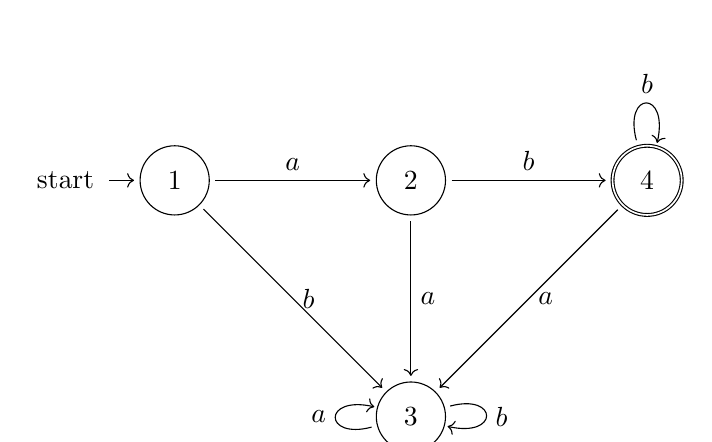
\begin{tikzpicture}[node distance=3cm, shorten >= 2pt, shorten <= 2pt]
        \node[initial, state] (1) {$1$};
        \node[state] (2) [right of=1] {2};
        \node[state] (3) [below of=2] {3};
        \node[state, accepting] (4) [right of=2] {4};

        \path[->] (1) edge [above] node [align=center] {$a$} (2)
                  (2) edge [above] node [align=center] {$b$} (4)
                  (1) edge [right] node [align=center] {$b$} (3)
                  (2) edge [right] node [align=center] {$a$} (3)
                  (4) edge [right] node [align=center] {$a$} (3)
                  (3) edge [loop right] node [align=center] {$b$} (3)
                  (3) edge [loop left] node [align=center] {$a$} (3)
                  (4) edge [loop above] node [align=center] {$b$} (4);
    \end{tikzpicture}
    \caption{DFA Example 1}
    \label{fig:dfa-string}
\end{figure}

The above diagram shows a transition diagram. A string which is translated into it is read from left to right, for example $abbb$ would be accepted as it finishes in the accept state however $abbab$ would not be as it finishes at node 3 not at the finish state.\\

A DFA's states are represented as circles (or other shapes for convenience when it's meaning is clear) in the transition diagram. A DFA begins in the initial state, denoted by the pointing into a shape - here the initial state is 1. It the reads the input string, one symbol at a time and for each symbol read it makes a transition to a new state according to the labelled arcs. One or more states can be accepting states - denoted by a double circle. Here only state 4 is an accepting state. If after reading the complete string, the DFA is in an accepted state - we say that the string is accepted and otherwise it is rejected.\\

DFAs are just another way to represent something that we could use a RegEx to represent. The RegExs:
\begin{align*}
    r &= abb^*\\
    r &= ab ^+
\end{align*}
could be used to represent the DFA shown above. 

\subsection{A More Mathematical Example...}
Considering the DFA that accepts strings of decimal digits containing a single decimal point:
\begin{figure}[H]
    \centering
    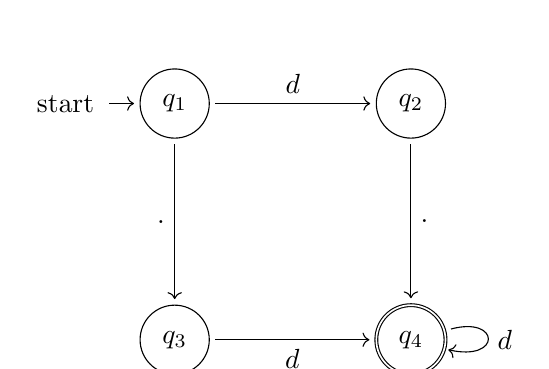
\begin{tikzpicture}[node distance=3cm, shorten >= 2pt, shorten <= 2pt]
        \node[initial, state] (1) {$q_1$};
        \node[state] (2) [right of=1] {$q_2$};
        \node[state] (3) [below of=1] {$q_3$};
        \node[state, accepting] (4) [below of=2] {$q_4$};

        \path[->] (1) edge[above] node[align=center] {$d$} (2)
                  (1) edge[left] node[align=center] {$.$} (3)
                  (3) edge[below] node[align=center] {$d$} (4)
                  (2) edge[right] node[align=center] {$.$} (4)
                  (4) edge[loop right] node[align=center] {$d$} (4);
    \end{tikzpicture}
    \caption{DFA Example 2}
\end{figure}

The DFA above is defined as:
\begin{align*}
    \Sigma &= \{1, 2, 3, 4, 5, 6, 7, 8, 9, .\}\\
    Q &= \{q_1, q_2, q_3, q_4\}
\end{align*}
$q_1$ is the initial stage, and $F=\{q_4\}$ is the set of final states. The transition functions can be represented by a set of triples:
\begin{align*}
    \delta = \{\quad &\\
        & (q_1, 0, q_2)., \ldots, (q_1, 9, q_2),\\
        & (q_1, ., q_3)\\
        & (q_2, 0, q_2), \ldots, (q_2, 9, q_2)\\
        & (q_2, ., q_4)\\
        & (q_3, 0, q_4), \ldots, (q_3, 9, q_4)\\
        & (q_4, 0, q_4), \ldots, (q_4, 9, q_4)\\
    \}\quad &
\end{align*}
In each triple $(q_i, a, q_j)$, $q_i$ is the current state, $a$ is the input and $q_j$ is the state which the DFA will transit to. For example: $\delta(q_i, a)=q_j$.

\section{Language of a DFA}
The set of all strings accepted by the DFA is known as the \textit{language recognised} by the DFA. This means that for a DFA, $M$, the language $L(M)$ is defined as `the set of all strings $w \in \Sigma^*$ such that when the DFA starts processing $w$ from its initial state it ends up in an accepting state'. \\

For example, the language for the string processing DFA (Fig \ref{fig:dfa-string}) is a set of strings:
\[L(M) = \{ab^n | n \geq 1\}\]

There are in fact algorithms that, given a regular expression $r$, builds a DFA (or NFA) $M$ such that:
\[L(M) = L(r)\]

\subsection{Simplification to DFA Diagrams}
We often have a large number of transitions between two states in a DFA. For example - in an identifier recognition DFA, there are 52 arcs for English letters (labelled by each of the lower and upper-case letters); and 10 for digits. Drawing that many transition arcs to a DFA is not a good choice. For this reason, we name a set of symbols:
\begin{align*}
    letter &= \{a,b,c,\ldots, z, A, B, C, \ldots, Z\}\\
    digit &= \{0, \ldots, 9\}
\end{align*}
and replace their arcs by a single arc labelled $letter$ or $digit$ (or simply $d$ as in our example).\\

Therefore, the regular expression
\[ident = letter (\_|letter | digit)^*\]
can be represented with the following DFA
\begin{figure}[H]
    \centering
    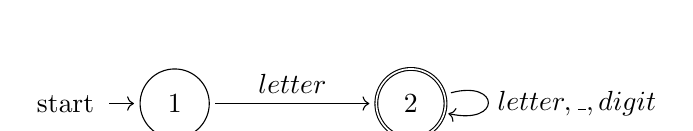
\begin{tikzpicture}[node distance=3cm, shorten >= 2pt, shorten <= 2pt]
        \node[initial, state] (1) {$1$};
        \node[state, accepting] (2) [right of=1] {$2$};
        
        \path[->] (1) edge[above] node[align=center] {$letter$} (2)
                  (2) edge[loop right] node[align=center] {$letter, \_, digit$} (2);
    \end{tikzpicture}
    \caption{Example DFA 3}
\end{figure}


\subsection{A More Sophisticated Example}
If we take the example of a DFA for the lexical analyser for a minimal language that includes:
\begin{itemize}
    \item identifiers
    \item the symbols: \verb|:=|, \verb|+|, \verb|;|
    \item keywords \verb|program|, \verb|begin|, \verb|end|, \verb|input| \& \verb|output|
\end{itemize}

It should output tokens \verb|END OF INPUT|, \verb|ERROR|, \verb|IDENTIFIER|, \verb|ASSIGN|, \verb|PLUS|, \verb|SEMI COLON|, \verb|PROGRAM|, \verb|BEGIN|, \verb|END|, \verb|INPUT| \& \verb|OUTPUT|\\

% DIAGRAM

The DFA begins in its initial state \verb|START|, and a token is recognised as soon as the accepting state \verb|DONE| is recognised. For example, if the arch labelled \verb|+| is taken, then token \verb|PLUS| has been  recognised. The re-read means that the input character resulted in this particular transition being taken should be read again (because it is the first character of the next token). The state names \verb|IN_ID| and \verb|IN_ASSIGN| can be replaced with any other meaningful names. 

\section{Building a Lexical Analyser}
Lexical analysers tend to be built in three ways:
\begin{enumerate}
    \item Write a formal definition of the token patterns, which are used as an input to a software tool (i.e. \textit{Lex}) which automatically generates a lexical analyse 
\end{enumerate}
or, design DFAs that describe the token patterns, then
\begin{enumerate}
    \setcounter{enumi}{1}
    \item write a program to implement the diagram
    \item write a table-driven implementation of the DFA.
\end{enumerate}
There are algorithms that construct lexical analysers from DFAs automatically.

\subsection{Lex}
The \textit{Lex} program is a lexical analyser generator. It was written in the 70s and new versions are available.
\begin{itemize}
    \item Flex: a variant of the classic ``lex'' (C/C++)
    \item JLex: lexical analyser generator for Java, written in Java
    \item Quex: A fast universal lexical analyser generator for C and C++
\end{itemize}
The program \textit{Lex} takes as input a source file (called a Lex file) comprising regular expressions for various tokens and automatically generates (most of) a lexical analyser in C. Therefore, the work of creating a lexical analyser using Lex is most about preparing Lex files.\\

In its most basic form - a Lex file comprises a series of lines of the form
\begin{verbatim}
    pattern                 action
\end{verbatim}
where \verb|pattern| is a regular expression and \verb|action| is a piece of code. For example the following is a complete Lex file that displays token names rather than returning tokens to the syntax analyser.
\begin{verbatim}
    %%
    [ \n\t]+                { ; }
    if                      { printf("IF\n"); }
    then                    { printf("THEN\n"); }
    [0-9]+                  { printf("NUMBER\n"); }
    [a-zA-Z][_0-9a-zA-Z]*   { printf("IDENT\n"); }
    .                       { printf("ERROR\n"); }
    %%
\end{verbatim}

The patterns on the left are all regular expressions, although in a slightly different notation to what has been discussed in this module so far. Running this Lex file on Lex produces a C file, which is then compiled by a C compiler to produce the lexical analyser. 
\taughtsession{Lecture}{Describing Language Syntax}{2024-02-16}{14:00}{Jiacheng}{}

\section{Context-Free Grammars}
The linguist Noam Chomsky introduced four classes of formal grammars for describing natural languages:
\begin{itemize}
    \item regular
    \item context-free
    \item context-sensitive
    \item recursively enumerables
\end{itemize}
Of the above listed, two have been found to be useful to describe programming languages:
\begin{itemize}
    \item regular grammars (equivalently, regular expressions) are useful for describing languages' lexical structure
    \item context-free grammars (CFG) for defining their syntax.
\end{itemize}

By far, CGF is the most widely used way to describe a programming language.

\subsection{What is A CFG?}
A CFG is a tuple: $G=(T,N,S,P)$ where:
\begin{itemize}
    \item[$T$] is a finite non-empty set of terminal symbols, which consist of strings in the language (for example \verb|while|), which refer to parts of the text of sentences in the language
    \item[$N$] is a finite non-empty set of non-terminal symbols, disjoint from $T$. These refer to syntactic structures defined by other structures and rules (for example \verb|<exp>|)
    \item[$S$] the start symbol, where $S \in N$
    \item[$P$] is a set of (context-free) productions of the form $A \rightarrow \alpha$ (which reads $A$ produces $\alpha$) where $A \in N$ and $\alpha \in (T \cup N)$
\end{itemize}

\subsection{Example of a CFG}
Taking the CFG as $G_1 = (T, N, S, P)$ where:
\begin{align*}
    T &= \{a, b\}\\
    N &= \{S\}\\
    P &= \{S \rightarrow ab, S \rightarrow aSb\}
\end{align*}
We know that this is a CFG because it has $T$ which is a set of symbols available in the language; $N$ containing the start-state (therefore non-terminal) $S$ and a set of rules of production $P$.\\

To take the CFG $G_2 = (T, N, S, P)$ where:
\begin{align*}
    T &= \{a,b\}\\
    N &= \{S,C\}\\
    P &= \{S \rightarrow \varepsilon, S \rightarrow C, S \rightarrow aSa, s \rightarrow bSb, C \rightarrow a, C \rightarrow b \}
\end{align*}

\subsection{Shorthand Notation}
It's lovely writing the CFGs out in full however this takes up quite a lot of space. So, instead of writing each individual rules of a given non-terminal, we are able to group the alternative right hand sides and separate them using $|$. For example, $G_2$ can be written as follows:
\begin{align*}
    S & \rightarrow \varepsilon | C | aSa | bSb\\
    C & \rightarrow a | b
\end{align*}

\subsection{Symbol Choice Conventions}
As we have seen in the above examples, there is a standard naming conventions for the symbols used:
\begin{itemize}
    \item $a, b, c, \ldots$ for members of $T$ (single terminal symbols)
    \item $A, B, C, \ldots$ for members of $N$ (single non-terminal symbols)
    \item $\ldots, X, Y, Z$ for members of $T \cup N$ (single symbols, terminal or non-terminal)
    \item $w, x, y, z, \ldots$ for members of $T^*$ (strings of terminal symbols)
    \item $\alpha, \beta, \gamma, \ldots$ for members of $(T\cup N)^*$ (mixed strings of terminals and / or non-terminal symbols)
\end{itemize}
Here $a, b, c, \ldots$ refer to letters at the beginning of the alphabet (the set of all symbols) and $w, x, y, z, \ldots$ to letters at the end of the alphabet.

\section{Backus-Naur Form (BNF)}
Backus-Naur Form (BNF) is a popular notation for CFG definitions of real programming languages. BNF uses angle brackets to denote non-terminal symbols, in a similar way to XML tags. For example \verb|<exp>|, \verb|<number>| and \verb|<digit>| are non-terminal; while \verb|+|, \verb|-|, \verb|*|, \verb|/|, \verb|0|, \verb|1|, \ldots{} \verb|9| are terminal symbols. 

\subsection{Syntactic Structures}
Using the above symbols, the syntactic structure for arithmetic expression would be defined by the following productions:
\begin{lstlisting}
    <exp> $\rightarrow$ <exp> + <exp> | <exp> + <exp> | 
             <exp> * <exp> | <exp> / <exp> | (<exp>) | <number>
    
    <number> $\rightarrow$ <digit> | <digit> <number>

    <digit> $\rightarrow$ 0 | 1 | 2 | 3 | 4 | 5 | 6 | 7 | 8 | 9 
\end{lstlisting}
    
In the above example, \verb|<exp>|, \verb|<number>| and \verb|<digit>| are non-terminals while \verb|+|, \verb|-|, \verb|*|, \verb|/|, \verb|0|, \verb|1|, \ldots{} \verb|9| are terminals. 

\subsection{Grammar for a Simple Language}
Below is a complete example of a BNF definition for a simple language:
\begin{lstlisting}
      <program> $\rightarrow$ begin <stmt-list> end
    <stmt-list> $\rightarrow$ <stmt> | <stmt> ; <stmt-list>
         <stmt> $\rightarrow$ <assign>
                   | <input-stmt>
                   | <output-stmt>
       <assign> $\rightarrow$ <ident> := <exp>
          <exp> $\rightarrow$ <ident> | <exp> + <exp>
   <input-stmt> $\rightarrow$ input <ident>
  <output-stmt> $\rightarrow$ output <ident>
        <ident> $\rightarrow$ x | y | z
\end{lstlisting}

\section{Derivations}
We can use a Context-Free Grammar to \textit{derive} strings of terminal symbols. Starting with the start symbol, $S$, we repeatedly apply the production rules until we obtain a string comprising only of terminal symbols, which is called a sentence. This process is called a derivation. Every string of symbols in a derivation is a sentential form. \\

The language defined by a grammar is made up of exactly those sentences that can be derived from it.
\subsection{An Example}
If we consider the grammar $G_2 (T, N, S, P)$ where:
\begin{align*}
    T &= \{a,b\}\\
    N &= \{S,C\}\\
    P &= \{S \rightarrow \varepsilon, S \rightarrow C, S \rightarrow aSa, s \rightarrow bSb, C \rightarrow a, C \rightarrow b \}
\end{align*}
We are able do derive the string $abbba$ for $G_2$ in the following steps:
\begin{enumerate}
    \item We begin with the start symbol $S$
    \item Applying the rule $S \rightarrow aSa$, we replace the $S$ by $aSa$ to obtain the string $aSa$.
    \item Applying the rule $S \rightarrow bSb$ on the new string $aSa$, we replace the $S$ by $bSb$ to obtain the string $abSba$
    \item Applying the rule $S \rightarrow C$, we obtain the string $abCba$
    \item Applying the rule $C \rightarrow b$, we obtain the string $abbba$ of terminal symbols.
\end{enumerate}

\subsection{Notation}
As we can see above, that is quite a long handed approach to righting out a derivation. There is a shorthand way of writing out a derivation as we will see below.\\

If we can get from $\alpha$ to $\beta$ by applying a single application rule, we say $alpha$ immediately derives $\beta$ written
\[\alpha \Rightarrow \beta\]
(note the double line'd arrow used here, not a single line as we have seen above for production rules)\\

We can therefore write the full derivation of $abba$ from $S$ as:
\begin{align*}
    S & \Rightarrow aSa\\
    & \Rightarrow abSba\\
    & \Rightarrow abCba\\
    & \Rightarrow abbba
\end{align*}

\subsection{Full Derivation Example}
We've now seen all the components to derivation, so now we will see a full example. The grammar of our language is as follows:
\begin{lstlisting}
    <program> $\rightarrow$ <stmts>
      <stmts> $\rightarrow$ <stmt> | <stmt> ; <stmts>
       <stmt> $\rightarrow$ <var> = <expr>
        <var> $\rightarrow$ a | b | c | d
       <expr> $\rightarrow$ <term> + <term> | <term> - <term>
       <term> $\rightarrow$ <var> | const
\end{lstlisting}
In the above grammar, \verb|<program>| is the start symbol, making it non-terminal; \verb|<stmt>|, \verb|<stmts>|, \verb|<expr>|, \verb|<term>|, and \verb|<var>| are non-terminals; whereas \verb|a|, \verb|b|, \verb|c|, \verb|d|, \verb|+|, \verb|-| and \verb|const| are terminals. \\

We can derive a single line program:
\begin{center}
    \verb|a = b + const|
\end{center}
from this grammar:
\begin{lstlisting}
    <program> $\Rightarrow$ <stmts>
              $\Rightarrow$ <stmt>
              $\Rightarrow$ <var> = <expr>
              $\Rightarrow$ a = <expr>
              $\Rightarrow$ a = <term> + <term>
              $\Rightarrow$ a = <var> + <term>
              $\Rightarrow$ a = b + <term>
              $\Rightarrow$ a = b + const
\end{lstlisting}
Lines 5 and 6 are in Sentential Form and the final line (ln. 8) is the finished sentence.\\

There is a second example of a derivation in the \verb|lecture06| slides on Moodle.

\subsection{Leftmost \& Rightmost Derivations}
Considering the following grammar for arithmetic expression
\begin{lstlisting}
    <exp> $\rightarrow$ <exp> + <exp> | <exp> * <exp> | x | y | z
\end{lstlisting}
A derivation of the sentence \verb|x + y * z| from this grammar could be:
\begin{lstlisting}
    <exp> $\Rightarrow$ <exp> + <exp>
          $\Rightarrow$ x + <exp>
          $\Rightarrow$ x + <exp> * <exp>
          $\Rightarrow$ x + y * <exp>
          $\Rightarrow$ x + y * z
\end{lstlisting}
Which is known as a \textit{leftmost} derivation because, at each step, the leftmost non-terminal symbol is resolved.\\

It is also possible to have a rightmost derivation:
\begin{lstlisting}
    <exp> $\Rightarrow$ <exp> + <exp>
          $\Rightarrow$ <exp> + <exp> * <exp>
          $\Rightarrow$ <exp> + <exp> * z
          $\Rightarrow$ <exp> + y * z
          $\Rightarrow$ x + y * z
\end{lstlisting}

It is also possible to have a neither left-nor right-most:
\begin{lstlisting}
    <exp> $\Rightarrow$ <exp> + <exp>
          $\Rightarrow$ <exp> + <exp> * <exp>
          $\Rightarrow$ <exp> + y * <exp>
          $\Rightarrow$ x + y * <exp>
          $\Rightarrow$ x + y * z
\end{lstlisting}

\section{Parse Trees}
We are able to illustrate the structure of an the expression given by a derivation as a parse tree.
\begin{figure}[H]
\centering
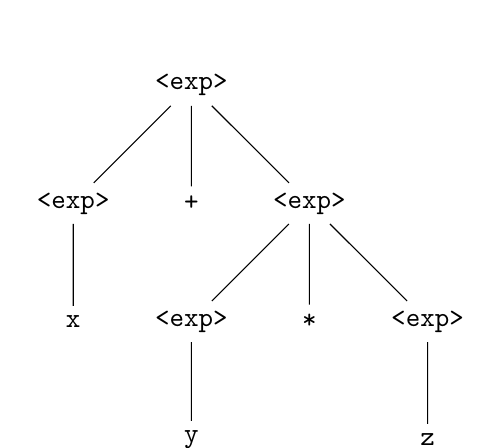
\begin{tikzpicture}[font=\ttfamily]
\node{<exp>}   
    child {node {<exp>}
        child {node {x}}}
    child {node {+}}
    child {node {<exp>}
        child {node {<exp>}
            child {node {y}}}
        child {node{*}}
        child {node {<exp>}
            child {node {z}}}};
\end{tikzpicture}
\caption{Parse Tree for derivation of \texttt{x + y * z}}
\end{figure}

The derivation of \verb|x = y * z| can be seen below
\begin{lstlisting}
    <exp> $\Rightarrow$ <exp> + <exp>
          $\Rightarrow$ x + <exp>
          $\Rightarrow$ x + <exp> * <exp>
          $\Rightarrow$ x + y * <exp>
          $\Rightarrow$ x + y * z
\end{lstlisting}

The internal nodes of the parse tree contin non-terminal symbols whereas leaf nodes contin terminal symbols. \\

It should be noted that for some grammars, the derivation of a given sentence can be different. Meaning they have different parse trees. This will commonly be the case when applying different ordered derivations.
\taughtsession{Lecture}{Syntax Analysis and Parsing}{2024-02-19}{1400}{Jiacheng}{}

\section{Ambiguities in Grammars}
Unsurprisingly, given the complex and custom nature of grammars - it is possible to make them ambiguous. This would mean that the derivation of given sentences could be different, therefore the parse trees are different.\\

For example if we take a left-most derivation for the sentence \verb|x + y * z|:
\begin{lstlisting}
    <exp> $\Rightarrow$ <exp> + <exp>
          $\Rightarrow$ x + <exp>
          $\Rightarrow$ x + <exp> * <exp>
          $\Rightarrow$ x + y * <exp>
          $\Rightarrow$ x + y * z
\end{lstlisting}
However, we can first apply the rule:
\begin{lstlisting}
    <exp> $\rightarrow$ <exp> * <exp>
\end{lstlisting}
which would yield:
\begin{lstlisting}
    <exp> $\Rightarrow$ <exp> * <exp>
          $\Rightarrow$ <exp> + <exp> * <exp>
          $\Rightarrow$ x + <exp> * <exp>
          $\Rightarrow$ x + y * <exp>
          $\Rightarrow$ x + y * z
\end{lstlisting}

These two derivations would produce different parse trees:
\begin{figure}[H]
\centering
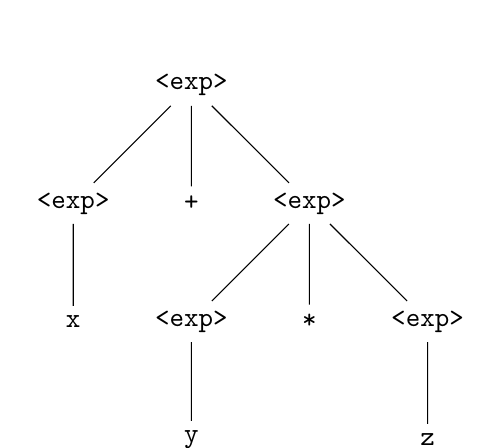
\begin{tikzpicture}[font=\ttfamily]
\node{<exp>}   
    child {node {<exp>}
        child {node {x}}}   
    child {node {+}}
    child {node {<exp>}
        child {node{<exp>}
            child {node {y}}}
        child {node {*}}
        child {node{<exp>}
            child {node{z}}}
    };
\end{tikzpicture}
\caption{Parse Tree for derivation of \texttt{x + y * z}}
\end{figure}

\begin{figure}[H]
\centering
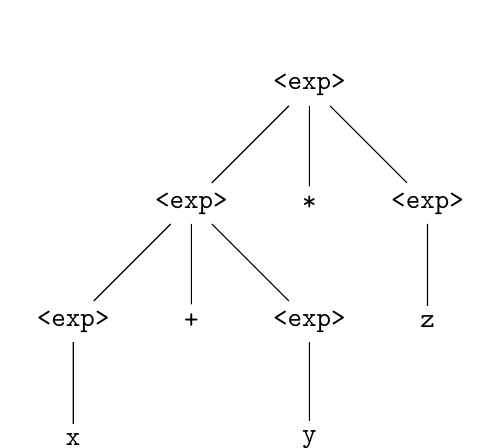
\begin{tikzpicture}[font=\ttfamily]
\node{<exp>}   
    child {node {<exp>}
        child {node{<exp>}
            child {node {x}}}
        child {node {+}}
        child {node{<exp>}
        child {node{y}}}}
    child {node {*}}
    child {node {<exp>}
        child {node {z}} 
    };
\end{tikzpicture}
\caption{Parse Tree for alternate derivation of \texttt{x + y * z}}
\end{figure}

An \textit{Abstract Syntax Tree} only shows the terminal symbols, without showing expressions. 

\begin{figure}[H]
\centering
\begin{tikzpicture}[font=\ttfamily]
\node{+}   
    child {node {x}}
    child {node {*}
        child {node {y}}
        child {node {z}}              
    };
\end{tikzpicture}
\caption{Example of an Abstract Syntax Tree}
\end{figure}
    

\subsection{Avoiding Ambiguity}
Ambiguity in grammars should be avoided, as we know from primary school - ambiguity in mathematical expressions has been removed through having an order of precedence which we can use brackets as part of.

\subsection{Removing Ambiguity}
For nearly all programming languages, the ambiguities in a grammar can be removed. To do this, extra non-terminals and rules are added. For example, taking the example grammar below:
\begin{lstlisting}
    <exp> $\rightarrow$ <exp> + <exp> | <exp> * <exp> | x | y | z
\end{lstlisting}
which can be disambiguated by adding rules that force certain operations (\verb|+|) to appear above other operators (\verb|*|) in parse trees. Thus giving the standard precedence of \verb|+| then \verb|*|. The new grammar can be seen below:
\begin{lstlisting}
       <exp> $\rightarrow$ <exp> + <term> | <term>
      <term> $\rightarrow$ <term> * <factor> | <factor>
    <factor> $\rightarrow$ x | y | z
\end{lstlisting}
Note that \verb|term| and \verb|factor| are newly introduced non-terminals.

\subsection{Limits of Context-Free Grammars}
There are some aspects of programming language syntax that cannot be captured using a context-free grammar. For example, the rule that variables must be declared before they are used is a \textit{context sensitive} property. Context-sensitive properties are resolved by the semantic analyser (which is beyond the scope of this module). 

\section{Syntax Analyser}
For any given input program, the goals of syntax analysis (also known as parsing) are to:
\begin{itemize}
    \item find all syntax errors, and for each discovered - produce an appropriate diagnostic message and recover quickly
    \item produce the parse tree for the program for code generation
\end{itemize}
These two functions are carried out by the syntax analyser (also known as the parser). There are different algorithms for parsing which are completed by different parsers.

\subsection{An Example}
If we take the grammar:
\begin{lstlisting}
    <exp> $\rightarrow$ <exp> + <exp> | <exp> * <exp> | x | y | z
\end{lstlisting}
the source code:
\begin{verbatim}
    x + y * z
\end{verbatim}
It will produce the tokens outputted by the scanner:
\begin{verbatim}
    IDENT PLUS IDENT MULTI IDENT
\end{verbatim}
And the following Parse Tree:
\begin{figure}[H]
\centering
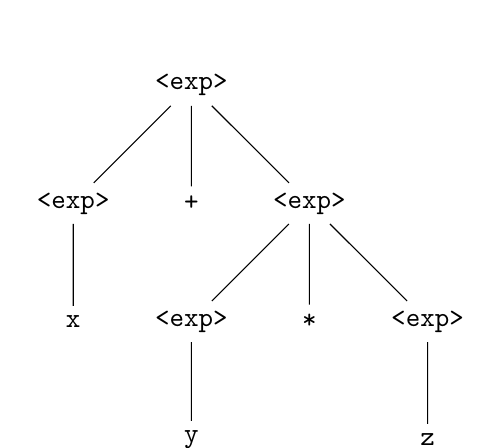
\begin{tikzpicture}[font=\ttfamily]
\node{<exp>}   
    child {node {<exp>}
        child {node {x}}}   
    child {node {+}}
    child {node {<exp>}
        child {node{<exp>}
            child {node {y}}}
        child {node {*}}
        child {node{<exp>}
            child {node{z}}}
    };
\end{tikzpicture}
\caption{Example Parse Tree for derivation of \texttt{x + y * z}}
\end{figure}
With the following abstract syntax tree:
\begin{figure}[H]
\centering
\begin{tikzpicture}[font=\ttfamily]
\node{+}   
    child {node {x}}
    child {node {*}
        child {node {y}}
        child {node {z}}              
    };
\end{tikzpicture}
\caption{AST For example}
\end{figure}

\section{Parsers}
There are two categories of parsers.\\

\textbf{Top-Down Parsers} begin with the root (the start symbol of the grammar rules) then visit each node (of the parse tree) before the branches are followed. For a left-most derivation, the branches from a given node are visited in left-to-right order.\\

\textbf{Bottom-Up Parsers} begin at the leaves of the parse tree (which are terminal symbols) and progress towards the root. The order is that of the reverse of a rightmost derivation.

\subsection{Parsing: An Example}
If we consider the following grammar:
\begin{align*}
    S & \rightarrow AB\\
    A & \rightarrow aA|\varepsilon \\
    B & \rightarrow b | bB
\end{align*}
The above grammar defines strings consisting of any number (0 included) of $a$'s followed by at least one (with the possibility of more) $b$'s. \\

If we consider parsing the string $aaab$ using the grammar by top-down parsing:
\begin{enumerate}
    \item begin with the start symbol $S$ and read the sentence one character at a time from the left
    \item at each step - expand the leftmost non-terminal by replacing it with the right side of one of its productions
    \item repeat until only terminals remain
\end{enumerate}
Shown below is the full parsing for the string:
\begin{itemize}
    \setlength{\itemindent}{2em}
    \item[$\boldsymbol{S}$] Begin with $S$ (start symbol)
    \item[$\boldsymbol{A}B$] $S \rightarrow AB$ (replace $S$ with the right hand side of $S \rightarrow AB$)
    \item[$a\boldsymbol{A}B$] $A \rightarrow aA$ (the leftmost non-terminal is $A$. On seeing first input $a$, replace $A$ with the right hand side of $A \rightarrow aA$)
    \item[$aa\boldsymbol{A}B$] $A\rightarrow aA$ (on seeing 2nd $a$)
    \item[$aaa\boldsymbol{A}B$] $A \rightarrow aA$ (on seeing 3rd $a$)
    \item[$aaa\varepsilon\boldsymbol{B}$] $A \rightarrow \varepsilon$ (on seeing $b$, use $A \rightarrow \varepsilon$ to make $A$ disappear as there is no rule for $A \rightarrow b$ and we can't work on non-terminal $B$ yet)   
    \item[$aaa\boldsymbol{B}$] 
    \item[$aaab$] $B \rightarrow b$ (on seeing $b$)
\end{itemize}

The top-down parse of the string $aaab$ is a left-most derivation of the sentence, which verifies that $aaab$ is a legal sentence. \\

At each step of top-down parsing:
\begin{itemize}
    \item Give a general sentential form, $xA\alpha$ where $x$ is a string of terminal symbols, $A$ is a non-terminal symbol and $\alpha$ is a mixed string of terminal \& non-terminal symbols. 
    \item This means that $A$ is the leftmost non-terminal that must be expanded to get the next sentential form in a leftmost derivation. 
    \item Determining the next sentential form is a matter of choosing the correct grammar rule that has $A$ as its left hand side. 
\end{itemize}
For example, with the current sentential form, $xA\alpha$, suppose the grammar has three rules for A:
\begin{align*}
    A & \rightarrow bB\\
    A & \rightarrow cBb\\
    A & \rightarrow a
\end{align*}
Depending upon the next input being $a$, $b$ or $v$, a top-down parser must choose among these three rules to generate the nex sentential form (from $xA\alpha$). 

\subsection{Predictive Parsers}
Different top-down parsing algorithms may use different information to make parsing decision (choosing the correct rules). Most parsers compare the next input token with the first symbols that can be generated by the right hand side of those rules, therefore called predictive parsers. A predictive parser is characterized by its ability to choose the production rule to apply solely based on the next input symbol and the current non-terminal being processed:
\begin{itemize}
    \item Current non-terminal $\Rightarrow$ choose the candidate rules
    \item Next input $\Rightarrow$ choose one rule among the candidates
\end{itemize}
Over this lecture and the next one, we will explore two different implementations of a predictive (top-down) parser.
\begin{itemize}
    \item Recursive descent parsers - a coded implementation of a syntax analyser based on BDF description of syntax
    \item LL (1) parsers - driven by a parsing table (created from BNF grammar) with: 1st L is a left-to-right scan of input; 2nd L is a leftmost derivation; and the `1' meaning one input symbol of lookahead (i.e. predictive)
\end{itemize}

\section{Recursive-Descent Parsers (RDP)}
A Recursive-Descent Parser (RDP) is made up of a collection of subprograms, many of which are recursive (hence where its name comes from) and produces a parse tree in top-down order.\\

Within an RDP - there is a subprogram for each non-terminal in the grammar. 

\subsection{RDP Example}
If we take the following grammar for a small set of simple expressions:
\begin{lstlisting}
       <exp> $\rightarrow$ <term> + <term> | <term> - <term>
      <term> $\rightarrow$ <factor> * <factor> | <factor> / <factor>
    <factor> $\rightarrow$ id | int_constant | (<exp>)
\end{lstlisting}

We can re-write the grammar for \verb|<exp>| and \verb|<term>| in a more compact form, because the only difference in the two alternatives in both cases is a terminal symbol (\verb|+| or \verb|-|, \verb|*| or \verb|/|):
\begin{lstlisting}
       <exp> $\rightarrow$ { ( + | - ) <term> }
      <term> $\rightarrow$ { ( * | / ) <factor> }
    <factor> $\rightarrow$ id | int_constant | (<exp>)
\end{lstlisting}

To implement a programmed recursive-descent parser, we need to implement three subprograms:
\begin{itemize}
    \item \verb|exp()|
    \item \verb|term()|
    \item \verb|factor()|
\end{itemize}
We would also assume that we have a lexical analyser (for example \verb|lex()|) that puts the next token in a variable called \verb|nextToken|. Upon receiving a token, the parser will decide:
\begin{itemize}
    \item if it is a terminal of current rule (i.e, \verb|+|, \verb|-|, \verb|*|, \verb|/|, \verb|id|, \ldots), continue to have the next token (make a call to \verb|lex()| to get \verb|nextToken|). 
    \item if it is a non-terminal symbol fo the right hand side of the current rule (i.e. \verb|<term>|, \verb|<factor>|), call it's associated parsing subprogram for that non-terminal
    \item if it is neither terminal nor non-terminal of the current rule or something else, then there is a syntax error.
\end{itemize}

\subsection{Rules with Multiple Right Hand Sides}
Where a rule ha multiple right hand sides, a decision has to be taken as to which one to use. The correct RHS could be chosen based on the next token of input - which is compared with the first token of each RHS until a match is found. If no match is found, it is a syntax error.
\taughtsession{Lecture}{LL1 Parsers}{2024-02-23}{1400}{Jiacheng}{}

\section{Top Down Parsing: Recursive Descent Parsers}
Last lecture, we saw the \textit{Recursive Descent Parsers} which are the coded implementation of a syntax analyser. We saw that the RDP consists of a collection of subprograms, and that there is a subprogram for each non-terminal in the grammar. Many of these subprograms are recursive, hence it's name. 

\section{Left Recursion Rules}
If a grammar makes uses of left recursion, either directly or indirectly, it cannot be used directly by a recursive-descent parse. A left recursion is where the definition is defined in terms of itself, for example $A \rightarrow A \alpha$. There are two different types of Left Recursion.
\begin{itemize}
    \item \textbf{Direct Left Recursion}, where the rule can directly invokes itself without making any progress in the parse string. For example:
    \[ A \rightarrow S \beta \]
    \item \textbf{Indirect Left Recursion}, where there are multiple stages to the left recursion as seen below:
    \begin{align*}
        S & \rightarrow A \beta \\
        A & \rightarrow S
    \end{align*}
\end{itemize}
Ultimately, left recursion leads to indefinite / non-terminating recursion. However, we are able to transform a left-recursive grammar into one that is not.

\subsection{Left Recursion Removal}
For each non-terminal involved in the Left Recursion,$A$, there are two steps which have to be undertaken. 
\begin{enumerate}
    \item Group the $A$-rules as: $A \rightarrow A\alpha_1 | \ldots A \alpha_m | \beta_1 | \beta_2 | \ldots | \beta_n $
    where $A \rightarrow A \alpha_1 | \ldots | A \alpha_m$ are rules with left recursion and $A \rightarrow \beta_1 | \beta_2 | \ldots | \beta_n$ are rules without left recursion.
    \item Introduce a new non-terminal, $A'$, and replace the original rules with:
    \begin{align*}
        A & \rightarrow \beta_1 A' | \beta_2 A' | \ldots | \beta_n A'\\
        A' & \rightarrow \alpha_1 A' | \alpha_2 A' | \ldots | \alpha_m A' | \varepsilon
    \end{align*}
\end{enumerate}

\section{Top Down Parsing: LL(1) Parsers}
LL(1) Parsers are table-driven Predictive Parsers. The LL(1) stands for the what the parser does:
\begin{itemize}
    \item 1st L: left-to-right scan of input.
    \item 2nd L: leftmost derivation
    \item ``1'': means one input symbol of lookahead
\end{itemize}

A LL(1) parser utilises: a \textit{stack} to store the symbols on the right-hand side of the productions in right-to-left order so that the leftmost symbol is on top of the stack; and a \textit{parsing table} which stores the actions (ie the rules) the parser should take based on the input token and what value is on top of the stack. 

\subsection{Example}
If we consider the following grammar:
\begin{align*}
    E & \rightarrow T\ E'\\
    E' & \rightarrow +TE' | \varepsilon\\
    T & \rightarrow FT'\\
    T' & \rightarrow *FT' | \varepsilon\\
    F & \rightarrow (E) | int
\end{align*}
Here, we have non-terminal symbols $E$, $T$ and $F$ which may stand for \verb|<exp>|, \verb|<term>|, \verb|<factor>| or other structures. $E$ is our start symbol.
\begin{table}[H]
\centering
\small
{\RaggedRight
\begin{tabular}{C{0.15\textwidth} C{0.11\textwidth} C{0.11\textwidth} C{0.11\textwidth} C{0.11\textwidth} C{0.11\textwidth} C{0.11\textwidth}}
\textbf{Top of parse stack} & \textbf{int} & \textbf{+} & \textbf{*} & \textbf{(} & \textbf{)} & \textbf{\$}\\
\hline
\hline
$E$ & $E \rightarrow TE'$ & & & $E \rightarrow TE'$ & & \\
\hline
$E'$ & & $E' \rightarrow +TE'$ & & & $E' \rightarrow \varepsilon$ & $E' \rightarrow \varepsilon$\\
\hline
$T$ & $T \rightarrow FT'$ & & & $T \rightarrow FT'$ & & \\
\hline
$T'$ & & $T' \rightarrow \varepsilon$ & $T' \rightarrow ^*FT'$ & & $T' \rightarrow \varepsilon$ & $T' \rightarrow \varepsilon$\\
\hline
$F$ & $F \rightarrow \mathrm{int}$ & & & $F \rightarrow (E)$ & & \\
\hline
\end{tabular}
} % end of rr     
\caption{Parse Table}
\end{table}

\begin{minipage}{0.2\textwidth}
    \begin{figure}[H]
        \centering
        \usetikzlibrary{shapes.multipart}
        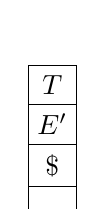
\begin{tikzpicture}[stack/.style={rectangle split, rectangle split parts=#1,draw, anchor=center}]
            \node[stack=4]  {
            \nodepart{one} $T$
            \nodepart{two}$E'$
            \nodepart{three}$\$$
            };
        \end{tikzpicture}
        \caption{Stack}
    \end{figure}
\end{minipage}\hfill
\begin{minipage}{0.75\textwidth}
    \begin{figure}[H]
        \centering
        \begin{tabular}[H]{| C{0.08\textwidth} | C{0.08\textwidth} | C{0.08\textwidth} | C{0.08\textwidth} | C{0.08\textwidth} | C{0.08\textwidth} | C{0.08\textwidth} | C{0.08\textwidth} |}
            \hline
            $($ & int & $+$ & int & $*$ & int & $\cdots$ & $\$ $\\
            \hline
        \end{tabular}
        \caption{Input Strings (tokens)}
\end{figure}
\end{minipage}

\subsection{Parsing Table}
For LL(1) parsing, the grammar is arranged into a parsing table.
\begin{itemize}
    \item The first column has the non-terminal symbols of the grammar,
    \item The first row contains the terminal symbols and $\$$ is for the end of input 
    \item The table entries give the rules of choice based on the current input (a terminal symbol) and the current non-terminal symbols (the symbol on top of the stack)
\end{itemize}

% ADD PARSING TABLE EXAMPLE

\subsection{Parsing Procedure / Algorithm}
Each step in parsing is about choosing a rule from the table according to the current non-terminal (which is on top of the stack) and current input; then pushing it's right-hand side into the stack. The $\$$ symbol represents the bottom of the stack. \\

The process begins with the start symbol ($E$ in our ongoing example). We push the right-hand side of the $E$ expression ($E \rightarrow TE'$) to into the stack, working right-to-left. This means that the top of our stack is now $T$.\\

Now, if we take the current input to be $int$. According to the table, $T \rightarrow FT'$ is selected and it's right hand side is pushed into the stack. Now the top of the stack is $F$.

% ADD TABLE
% ADD STACK EXAMPLES 
\taughtsession{Lecture}{Syntax Analysis - Bottom Up Parsing}{2024-03-01}{1400}{Jiacheng}{}

\section{Parse Table Construction}
LL(1) parse is easy if the action table is available. The construction of the action table of the LL(1) parser requires computing the first and follow sets (sets of non-terminal symbols) of the non-terminals of the grammar. \\[1em]

\textit{NB: There's lots of information on how the First sets of Non-Terminals work on the slides on Moodle.}

\section{Bottom-Up Parsing}
Bottom-Up parsing works in the opposite direction of top-down parsing. This means that it will start with the string of terminal symbols and then works backwards to the start symbol by applying the productions in reverse. 

\begin{enumerate}
    \item Begin with the rightmost symbol fo the sentence of terminals
    \item Apply a production in reverse at each step
    \item Replace a substring with the non-terminal on the left of a production whose right side matches the substring
    \item Continue until we have substituted our way back to the start symbol
\end{enumerate}

For example, using the following grammar:
\begin{align*}
    S & \rightarrow AB \\
    A & \rightarrow aA | \varepsilon \\
    B & \rightarrow b | bB
\end{align*}

We can then follow the parsing through:
\begin{itemize}
    \setlength{\itemindent}{2em}
    \item[$aaa\boldsymbol{b}$] (the sentence of terminals)
    \item[$aaa\boldsymbol{B}$] $B \rightarrow b$
    \item[$aaa\boldsymbol{\varepsilon}B$] (insert $\varepsilon$ because $a$ or $aB$ is not RHS of any rule)
    \item[$aa\boldsymbol{aA}B$] $A \rightarrow \varepsilon$
    \item[$a\boldsymbol{aA}B$] $A \rightarrow aA$ (we cannot use $S \rightarrow AB$ yet because it terminates the parsing with some terminal symbols not being parsed)
    \item[$\boldsymbol{aA}B$] $A \rightarrow aA$
    \item[$\boldsymbol{AB}$]  $A \rightarrow aA$
    \item[$\boldsymbol{S}$] $S \rightarrow AB$
\end{itemize}
An example of parsing the same string with Top-Down Parsing is available in the \textit{Parsing and Syntax Analysis} lecture.

\section{Top-Down vs Bottom-Up}
Bottom-Up parsing algorithms are more powerful than top-down methods. There are excellent parser generators like \textit{yacc} that build a parser from an input specification (a bit like how \textit{lex} builds a scanner). 

\section{Shift-Reduce Parsing}
Shift-Reduce Parsing is a bottom-up parsing technique which takes an input as a stream of tokens and develops the list of productions (the grammar rules) that are used to build the parse tree. It makes use of a stack to keep track of the position in the parsing process and a parsing table to determine what to do next. \\

Shift-Reduce parsing is the most used and most powerful bottom-up parsing techniques.

\subsection{The LR Parser}
The LR parser is a type of shift-reduce parser which scans the input from left-to-right and operates using a reversed rightmost derivation.\\

The LR Parser works as follows
\begin{itemize}
    \item When parsing a string of tokens $v$, the input is initialised to $v$ (ended with the end-marker $\$$) and the stack is initialised to empty. 
    \item Parsing starts by shifting the first (leftmost) token to the top of the stack
    \item A shift-reduce parser proceeds by taking one of three actions at each step
    \begin{description}
        \item[shift] where we transfer a token from the input onto the stack. In an ideal world, we would want to run a reduce or acceptance however if neither are possible - we run a shift. 
        \item[reduce] where we apply the production for a non-terminal backwards (replacing the RHS with the LHS of a grammar rule). For example if we have a production $A \rightarrow w$, we can produce $A$ from any $w$s we have at the top of the stack
        \item[acceptance] where we reduce the entire contents of the stack to the start symbol, with no remaining input means the input is a valid sentence. We would then say that the string is ``accepted''.
    \end{description}
    \item If none of the above cases apply, we have an error. An error is a case where we have a sequence on the stack that cannot eventually be reduced to the LHS of any production; and any further shift would be futile and the input cannot form a valid sentence.
\end{itemize}
\taughtsession{Lecture}{Exam Preperation}{2024-03-11}{0900}{Tobi}{}

\section{Exam Preparation}

\begin{itemize}
    \item The exam will cover content from week 1 through 5 (inclusive); there will be some vulnerabilities from week 1 and 2, however.
    \item The ultimate aim of the exam is to break the machines to Root access, and there will be a number of questions on Moodle which we will need to answer, some of these will be flag-style and some will require research on the machines and providing an answer.
    \item The `playbook' should contain details on some of the OWASP Top 10
    \item Some geolocation will be expected in the exam
    \item Filtered internet access will be provided, we will be provided with a list of of sites which we can access
    \item We will be breaking a webserver. There might be \textit{other} stuff running on it, however it will definitely be a webserver
    \item The webserver might be running WordPress, it might not.
    \item We will be provided with the \textit{rockyou} wordlist. If an attack using a wordlist is taking a long time then we should assume that it will not provide us the answer.
    \item If a hashcat is taking a long time, we should try other things while it is running
\end{itemize}
\taughtsession{Lecture}{Elementary Data Types}{2024-03-15}{14:00}{Jiacheng}{}

Elementary Data Types have fixed values that can be stored in a memory space of fixed size. Typically, languages provide the following kinds of elementary types:
\begin{itemize}
    \item Numeric (these are integer / floating points)
    \item Boolean
    \item Character
    \item Enumerated
    \item Reference or pointer
\end{itemize}
We will not look at all of these data types in great detail. \\

Imperative languages provide built-in operators for computing over these elementary data types. A selection of these operators is provided in the table below.

\begin{table}[H]
    \centering
    {\RaggedRight
    \begin{tabular}{p{0.3\textwidth} p{0.2\textwidth} p{0.2\textwidth} p{0.2\textwidth}}
    \textbf{Kind of Operator} & \textbf{Pascal} & \textbf{Python} & \textbf{C}\\
    \hline
    \hline
    Arithmetic & \verb|+ - * /| & \verb|+ - * /| & \verb|+ - * /|\\
    \hline
    Int division & \verb|div mod| & \verb|/ %| & \verb|/ %|\\
    \hline
    Relational \verb|= < >| \verb|< <= > >=| & \verb|== !=| \verb|< <= > >=| & \verb|== != < <= > >=|\\
    \hline
    Boolean & \verb|and or not| & \verb|and or !| & \verb+&& || !+\\
    \hline
    Bitwise & \verb|-| & \verb+& |+ & \verb+& |+\\
    \hline
    \end{tabular}
    } % end of rr     
    \caption{Operations on Elementary Data Types}
\end{table}

\section{Enumerated Types}
Enumerated types are \textit{ordinal} type that the possible values can be associated with the set of positive integers. Enumerated types are used to represent order, for example used as indices of arrays.\\

In Java - the primitive ordinal types are integer and char. The char data type is a single 16-bit Unicode character, which has a minimum value of `\textbackslash u0000' (or 0) and a maximum value of `\textbackslash uffff' (or 65,535). \\

Enumerated types can be user-defined. For example, if we wanted to define a type to represent the four seasons in Pascal:
\begin{verbatim}
    type season = (spring, summer, autumn, winter);
\end{verbatim}
We can then declare a variable of type \verb|season|:
\begin{verbatim}
    var s : season;
\end{verbatim}

\subsection{Operations}
Typically, enumerated types have a small set of operations - comparison and retrieval of the value of successor / predecessor value. We can see this in Java, which has included Enumerated Types (\verb|enum|) since version 1.5. The example below defines an \verb|enum| type \verb|Season| and then sets \verb|s| and displays the ordinal of it.
\begin{verbatim}
    public enum Season {SPRING, SUMMER, AUTUMN, WINTER};
    Season s = Season.SUMMER;
    System.out.println(s.ordinal()); // outputs '2'
\end{verbatim}

\section{Pointers}
Pointer (or reference) variables have a memory address as their value (they ``point'' to another data item). Originally, pointers were designed to work with memory locations, enabling efficient use of limited memory space - a feature of assembly language. They provide a convenient way to manage (allocate and de-allocate) dynamic storage (heap memory). Memory spaces that are dynamically allocated from a heap are heap-dynamic variables. They often are anonymous (meaning they do not have identifiers associated with them) and thus can be referenced only be pointers (memory addresses). C and C++ natively include lots of support for pointers.

\subsection{Pointer Type Declaration}
The declaration of a pointer is given by preceding a variable name with a \verb|*|:
\begin{verbatim}
    int number, *numPtr;
\end{verbatim}
The above code snipped declares \verb|number| as an \verb|int| and \verb|numPtr| as a ``pointer to int''. At runtime, this means:
\begin{itemize}
    \item \verb|number| is the name of a location in memory where an integer is stored
    \item \verb|numPtr| is the name of a location in memory where a memory address is stored.
\end{itemize}

\subsection{``\&'' Operator}
The \verb|&| operator retrieves the address of a variable. This can be used as follows:
\begin{verbatim}
    number = 42;
    numPtr = &number;
\end{verbatim}
whee the value of \verb|numPtr| is the address of variable \verb|number|. 

\subsection{Pointer Dereferencing}
The dereferencing operator (\verb|*|) of pointers to access the value pointed to by a pointer, for example if we wanted to print the value:
\begin{verbatim}
    printf("%d\n", *numPtr);
\end{verbatim}
The dereferencing operator is also used ot modify the value of the memory location that the pointer points to:
\begin{verbatim}
    *numPtr = 7
\end{verbatim}
The line above updates the value pointed to by \verb|numPointer| to be the value \verb|7|. 

\subsection{Null Pointers}
A special value \verb|null| (actually stored as \verb|0|) is assigned to pointer variables to signify that it doesn't point to any location. For example:
\begin{verbatim}
    numPtr = null;
\end{verbatim}
results in \verb|numPtr| not actually pointing to anything.

\subsection{Assignments Involving Pointers}
If we take the following code:
\begin{verbatim}
    int *p;
    int *q;
    int a = 100;
    p = &a;

    *q = *p;
\end{verbatim}
The code above involves pointer de-referencing, whereby it copies the content of the memory location pointed to by \verb|p| (\verb|100|) to the location pointed to by \verb|q|. This is distinctly different to the line
\begin{verbatim}
    q = p;
\end{verbatim}
which copies the value of \verb|p| (a memory address) to \verb|q|.

\subsection{Dynamic Memory Allocation}
Pointers are commonly used with dynamic memory allocation (where the memory allocation takes place at runtime). The following code allocates 400 bytes (100 spaces of 4 bytes each) and sets the variable \verb|data| to point to the first byte. Note that both of the first lines below do effectively the same thing:
\begin{verbatim}
    int *date = calloc(100, sizeof(int));
    int *data = malloc(400);
\end{verbatim}
There is, however, a difference between \verb|malloc| and \verb|calloc|
\begin{description}
    \item[calloc] allocates a block of memory of ``n elements'', each of \verb|sizeof| bytes and initializes the contents of the memory to zeroes. It contains info about memory organisation. Example above has created an integer array of 100 elements.
    \item[malloc] allocates specified size, with no organisation information, of memory however does not erase the memory space. This may lead to the memory containing garbage values.
\end{description}

\subsection{Semantics of Pointer Allocation}
When reading pointer arithmetic, it's important to understand it with reference to the pointer type on which they operate. For example:
\begin{verbatim}
    int *p;
    int *q;
    p = (int *) malloc(sizeof(int));
    q = (char *) malloc(sizeof(char));
    p = p + 1;
    q = q + 1;
\end{verbatim}
If two \verb|malloc| functions return \verb|addr1| for \verb|p| and \verb|addr2| for \verb|q|, after the increment operations - then the values of \verb|p| and of \verb|q| are not \verb|addr+1| and \verb|addr2+1| but instead are \verb|addr1+sizeof(int)| and \verb|addr2+sizeof(char)|. 

\subsection{Array Indices and Pointers}
Arrays in C are essentially pointers to large blocks of memory. For example, if we take:
\begin{verbatim}
    int a[10], *iPtr, sum, i;
    iPtr = &a[0];
\end{verbatim}
It would then be possible to access the individual elements of the array by using the indices of the array:
\begin{verbatim}
    a[0], a[1], a[2], ..., a[9]
\end{verbatim}
or by dereferencing the pointers:
\begin{verbatim}
    *(iPtr + 0),*(iPtr + 1), *(iPtr + 2),..., *(iPtr + 9) 
\end{verbatim}
This means the the following two for loops have the same effect\\

\begin{minipage}{0.45\textwidth}
\begin{verbatim}
for(i = 0, sum = 0; i < 10; i++){
    sum += a[i];
}
\end{verbatim}
\end{minipage}\hfill
\begin{minipage}{0.45\textwidth}
\begin{verbatim}
for(i = 0, sum = 0; i < 10; i++){
    sum += *(iPtr + i);
}
\end{verbatim}
\end{minipage}
\vspace{1em}

It is also possible to use indices on pointers:
\begin{verbatim}
    iPtr[2] is the same as
    *(iPtr + 2)
\end{verbatim}

When an array is declared ,the memory is allocated and the array name holds the address to the first byte of this block of memory. The name of the array is like a pointer which points to the first element of the array (for example \verb|a=&a[0]|)
\begin{verbatim}
    int a[10];
    int *iPtr;
    iPtr = a + 2;
\end{verbatim}
The last statement is the same as saying:
\begin{verbatim}
    iPrt = &a[0] + 2;
\end{verbatim}

it is also possible to do pointer arithmetic with array names. From this we can see that the following two statements are equivalent:
\begin{verbatim}
    *(a + 2) = 11;
    a[2] = 11;
\end{verbatim}

\subsection{Memory Deallocation}
Deallocation of memory can be explicit or implicit
\begin{verbatim}
    int *p = (int *) malloc (sizeof(int));
    *p = 5;
    p = null;
\end{verbatim}
In the above example, we see that assigning \verb|null| to \verb|p| destroys the only way to access the allocated memory (which is still in existence). The runtime environment can recognise the inaccessibility of this piece of memory and free it implicitly (through a process called garbage collection).\\

However, it is also possible to explicitly deallocate memory using the \verb|free(p)| statement as seen below:
\begin{verbatim}
    int *p = (int *) malloc(sizeof(int));
    int *q;
    *p = 5;
    q = p;
    free(p);
    p = null;
\end{verbatim}
It is regarded as good practice to assign \verb|null| to \verb|p| after freeing it. Note that it is a semantic error (with an unpredictable result) to invoke \verb|free| on a pointer which does not point to an object allocated using \verb|malloc|

\subsection{Dangling Pointers}
Taking the above example, after freeing \verb|p| - the pointer \verb|q| points to a heap-dynamic variable that has been deallocated. \verb|q| becomes a \textit{dangling pointer} that can cause unexpected errors at runtime. Another example:
\begin{verbatim}
    int *arrayPtr1;
    int *arrayPtr2 = new int[100];
    arrayPtr = arrayPtr2;
    delete [] arrayPtr2; // returns memory to heap
\end{verbatim}
Now, \verb|arrayPtr1| is dangling because the heap storage to which it was pointing has been deallocated.
\taughtsession{Lecture}{Compound \& Composite Data Types}{2024-03-22}{14:00}{Jiacheng}{}

A \textit{compound data type} is any data type which can be constructed using a programming languages' primitive data types. Common examples of compound types include: arrays, string, records, structs and variant records. Note that \textit{records} aren't directly found in OO languages, rather classes can be seen as extensions of records.

\section{Arrays}
The \textit{array} is the most common compound type found in programming languages. Generally speaking, an array has the following attributes:
\begin{itemize}
    \item The \textit{type} of its elements. This is also the type of the composite type
    \item The type of its \textit{indices}. Integers are normally used, however it is possible to use other types (for example, enumerated type)
    \item The \textit{index range} (number of elements)
\end{itemize}

As could be expected, the syntax and characteristics of arrays vary from language to language.

\subsection{Arrays in Different Languages}
We will consider two languages, Java and Pascal, to explore the differences between different languages implementations of arrays.\\

The first major difference is that in Pascal, the \textit{size} and \textit{indices} of an array oare part of it's type definition, for example:
\begin{verbatim}
    var rainfall: array [11 .. 20, 1..5] of real;
\end{verbatim}
The type of the variable \verb|rainfall| is an array of \verb|reals| indexed by integers between 11 and 20 (1st dimension), and between 1 and 5 (2nd dimension).\\

Pascal arrays allow any ordinal type as its indices, for example the enumerated type as indices:
\begin{verbatim}
    type month = (jan, feb, march, ..., dec);
    var rainfall : array [jan .. dec] of real;
\end{verbatim}
Or characters (128 ASCII characters, or 256 ANSI256 characters) as indices
\begin{verbatim}
    var anArray : array ['a' .. 'z'] of integer;
\end{verbatim}
Whereas in Java, arrays use integer type as its index and the index always starts from \verb|0|:
\begin{verbatim}
    double[] rainfall;
\end{verbatim}
Java supports a number of different index sizes:
\begin{itemize}
    \item Short (16-bit signed, -32768 to 32767)
    \item Byte (-128 to 127)
    \item Char (2 bytes, 65535)
\end{itemize}
These smaller types can be promoted (converted) to Integers which are bigger.

\subsection{Static v Dynamic Arrays}
As we saw in the Pascal definition example above, we now that the sizes of Pascal arrays are fixed at \textit{compile} time. We say that Pascal arrays are ``static''. By contrast, we saw that Java allows ``dynamic'' arrays. This means their sizes are determined at \textit{run-time} when they are created. For example:
\begin{verbatim}
    rainfall = new double[numDays];
\end{verbatim}

Dynamic arrays have the obvious advantage of allowing for the creation of more suitably-sized arrays.

\subsubsection{Static Arrays}
The subscript ranges (size of arrays) are statically bound and storage allocation is static at compile time. For example, all Pascal Arrays or C/C++ arrays which include the \verb|static| modifier. A key advantage is that they are more efficient as there is no dynamic allocation.

\subsubsection{Stack-Dynamic Arrays}
The subscript ranges are dynamically bound and the storage is allocated at run-time. It lives on the stack and the size of it is fixed once it is created. For example, C/C++ arrays without the \verb|static| modifier:
\begin{verbatim}
    double balance [100]; 
    myType stackArray[100];
\end{verbatim}
A key advantage is that dynamic arrays are more flexible (as the size of an array need not be known until the array is to be used). 

\subsubsection{Heap-Dynamic Arrays}
As the name would suggest, a heap-dynamic array lives on the heap. This means that it's size can change. C++, JavaScript, Python, etc support Heap-Dynamic arrays. For example, in C++:
\begin{verbatim}
    myType *heapArray = new myType[100];
    delete [] heapArray;
\end{verbatim}
A key advantage is that the Heap-Dynamic arrays are hugely flexible, meaning that they can grow or shrink during program execution.

\subsubsection{Java Arrays}
Java Arrays are objects and live on the heap (in the same way that other Java objects do), but they behave like stack-dynamic arrays. It's seen that they have fixed sizes once initialised:
\begin{verbatim}
    int [] a_array = new int (100);
\end{verbatim}

\subsection{Heterogeneous Arrays}
A \textit{heterogeneous} array is one in which the elements do not need to be of the same type. They are supported by Perl, Python and JavaScript. Shown below is an example of a heterogeneous array in JavaScript:
\begin{verbatim}
    var mixArray1 = new Array();
    mixArray1 [0] = "Hello, World!";
    mixArray1 [1] = 100;
\end{verbatim}
As would be expected, a heterogeneous array can be an element of another heterogeneous array:
\begin{verbatim}
    var mixArray2 = new Array(
        200,
        300,
        "Hello Again",
        mixArray1
    );
\end{verbatim}

\subsection{Rectangular \& Jagged Arrays}
A rectangular array is a multi-dimensional (for example, 2D) array in which all the rows have the same number of elements and all the columns have the same number of elements. This is supported by Fortran and C\#. (Note that C\# also supports jagged arrays).\\

A jagged array has rows with varying number of elements, however has no concept of columns. Therefore jagged multiple-dimensional arrays are actually arrays of arrays. C, C++, C\# and Java support jagged arrays. For example, a jagged array in Java:
\begin{verbatim}
    int [] [] myArray = { { 3, 4, 5 }, { 6, 7 } };
\end{verbatim}
Jagged arrays are more flexible and memory efficient. For example the second dimension of array \verb|a| can be allocated separately:
\begin{verbatim}
    int[][] a = int[3][];
    a[0] = new int[1]; // row 1 has 1 element
    a[1] = new int[2]; // row 2 has 2 element
    a[2] = new int[3]; // row 3 has 3 elements
\end{verbatim}
If \verb|a| turns out to be a big triangular array, almost half of the memory space can be saved by using a Jagged Array.

\section{Strings}
\textit{Strings} can be regarded as arrays / collections of characters.\\

In (standard) Pascal, strings need to be declared as arrays:
\begin{verbatim}
    var arr : packed array [1 .. 10] of char;
\end{verbatim}
\verb|packed| tells the compiler to use the minimum amount of memory.\\

In C, strings are declared as arrays:
\begin{verbatim}
    char name[10]; // memory allocated
\end{verbatim}
or as pointers to character:
\begin{verbatim}
    char *name; // memory not yet allocated
\end{verbatim}

In modern languages, strings are viewed as important enough to be built-in and a set of typical operations are defined for the string type such as:
\begin{itemize}
    \item finding the length / size of a string
    \item string concatenation
\end{itemize}
Note that the char array in C does not have these operations built in. 

\section{Record}
A \textit{record} is composed of a number of named elements of data. For example in Pascal:
\begin{verbatim}
    type date = record
        day: integer;
        month: integer;
        year: integer;
    end;
\end{verbatim}

We can see below how a variable \verb|d| is declared to be of type \verb|date|:
\begin{verbatim}
    var d: date;
\end{verbatim}
and how this has the \textit{fields} \verb|day|, \verb|month| and \verb|year|, which are accessed and modified using the dot notation / operator:
\begin{verbatim}
    writeln(d.year);  // access
    d.day = 24;       // modify
\end{verbatim}

\subsection{Structs}
A similar similar to record in C (and C++) are called \textit{structs}, for example:
\begin{verbatim}
    struct date {
        int day;
        int month;
        int year;
    }
\end{verbatim}
However! A struct in C++ is more powerful, as they may include \textit{member functions}:
\begin{verbatim}
    struct date {
        int day;
        int month;
        int year;
        void display();
    }
\end{verbatim}
As we can see above, it only declares the member function \verb|display()|, which means it will need to be defined elsewhere in the program. To display a date, we might call:
\begin{verbatim}
    date d;
    d.display();
\end{verbatim}

\subsection{Structs vs Classes}
Structurally, structs are similar to classes (without constructors) and member functions is an alternative term for method. A C++ class is shown below:
\begin{verbatim}
    class Date {
        int day;
        int month;
        int year;
    public:
        Date (int, int, int);  // constructor
        void display();
    }
\end{verbatim}
Another difference between structs and classes in C++ is that, by default, members are public in structs and private in classes.

\subsection{Whats the difference: Records, Structs \& Classes}
A Class is the concept of an Object Oriented language. It would be considered as an extension of records, given that procedural languages typically have records (containing fields), and object oriented languages have classes that contain fields (attributes) and methods (operators). 

\subsection{Variant Records}
Records can be inflexible and memory-inefficient, because all values of a record type have a fixed set of fields. For example, if we are creating a record to store students in; containing name, registration number, graduation status; then if they've graduated also storing their year of graduation and if not, storing their course number and year of enrolment.\\

Depending on the implementation of this, it could result in wasted fields which must be present in each record even if they're not needed.\\

However, in such cases - Pascal provides a \textit{variant record} to implement the alternative choices:
\begin{verbatim}
    type student = record
        name: array [1..30] of char;
        reg_no: integer;
        case graduated: boolean of;
        true (year_of_grad: integer);
        false (course_no: integer;
               year_of_enrol: integer);
    end;
\end{verbatim}

In the above example, we used a \verb|boolean| as the tag to determine which fields to include - other types (for example \verb|byte|) can be used in circumstances where we need more than two cases.

\subsection{Unions}
C \& C++ makes use of ``Unions'' instead of ``Variant Records''. Unions are designed for storing data items of multiple types in the same memory space. For example in C:
\begin{verbatim}
    typedef enum (INTEGER, DOUBLE) MyType;

    typedef struct {
        MyType a_type;
        union {
            int i;
            double d;
        } myUnion;
    } Value;
\end{verbatim}
Then we can either use the integer value:
\begin{verbatim}
    Value v;
    v.a_type = INTEGER;
    v.myUnion.i = 5;
\end{verbatim}
or we can use the double value:
\begin{verbatim}
    Value v;
    v.a_type = DOUBLE;
    v.myUnion.d = 5.4321;
\end{verbatim}

Here, we see that union is the storage for either an integer or a double but not both at the same time.

\subsection{Variant Records vs Union}
The main difference between the C implementation and the Pascal version is that in the C version (Union), it is possible to have both options set at the same time. This not the case in Pascal's Variant Records.
\taughtsession{Lecture}{Expression and Assignment}{2024-04-15}{14:00}{Jiacheng}{}

\section{Expressions}
An \textit{expression} is a combination of values ,variables, operators and function calls. Expressions perform operations on data and move data around. Expressions can be of the type:
\begin{itemize}
    \item arithmetic (\verb|4 * I + func(5)|)
    \item relational (\verb|a >= b|)
    \item boolean (\verb|A && B|)
    \item assignment (\verb|i = 4|)
\end{itemize}

Some expressions are very important and some of them are instrumental for implementing various algorithms. To correctly evaluate the expressions we need to know the rules of precedence and rules of associativity of operators.

\subsection{Arithmetic Expressions}
Arithmetic evaluation was one of the motivations for the development of the first programming languages. Arithmetic expressions consist of:
\begin{itemize}
    \item operators
    \item operands
    \item parentheses
    \item function calls
\end{itemize}

\section{Operators}
A \textit{unary} operator has one operand. For example:
\begin{itemize}
    \item The Negation operator ``\verb|-|'', used as \verb|-b| where \verb|-| is the operator and \verb|b| is the operand
    \item The \textit{Integer Promotion} operator ``\verb|+|'', used as \verb|+b| converts \verb|b| to \verb|int| if it is a \verb|short|, \verb|byte| or \verb|char|. 
\end{itemize}

WheWhen the operators \textit{precede} (or \textit{follow}) their operands, we say that the operators are ``prefix'' ()

When the operators precede their operands, we say the operators are ``prefix''; and when the operators follow follow their operands, we say the operators are ``postfix''. Unary operators can be prefix or postfix. For example the increment operator \verb|++| can either be used as \verb|i++| or \verb|++i|. A Binary operator has two operands - for example \verb|+|, \verb|-|, \verb|*|, \verb|/|. In most languages, binary operators are ``infix'' which means they appear between the operands.

\subsection{Operator Precedence Rules}
The \textit{operator precedence rules} define the order in which operations are evaluated within an expression. Typical precedence levels (from high to low) are shown below, with examples in brackets:
\begin{itemize}
    \item Parentheses (\verb|(| and \verb|)|)
    \item Unary Operators (\verb|++| and \verb|--|)
    \item Unary Operators (\verb|+| and \verb|-|)
    \item Binary Operators (\verb|*| and \verb|/|)
    \item Binary Operators (\verb|+| and \verb|-|)
\end{itemize}

\subsection{Operator Associativity Rules}
The operator associativity is a property that determines how operators of the same precedence are grouped in the absence of parentheses. For example, in the expression \verb|3/5*0|, operand \verb|5| is preceded and followed by operators \verb|/| and \verb|*| (which both have equal precedence). Which operator to apply to the operand is determined by the associativity of the operators. The operators may be:
\begin{description}
    \item[associative] the operations can be grouped arbitrarily. For example \verb|a * b * c| could be grouped as \verb|(a * b) * c| or as \verb|a * (b * c)|
    \item[left-associative] the operations are grouped from the left
    \item[right-associative] the operations are grouped from the right 
\end{description}

If we consider the expression \verb|a - b - c|. If the operator has left associativity, this expression would be interpreted as \verb|(a - b) - c|. Whereas if the operator has right associativity, this expression would be interpreted as \verb|a - (b - c)|.\\

However, it should be noted that some mathematical operators have inherent associativity. For example:
\begin{itemize}
    \item Subtraction (\verb|-|) and division (\verb|/|) are inherently left-associative
    \item Addition (\verb|+|) and multiplication (\verb|*|), by contrast are both left and right associative.
\end{itemize}

Many programming language manuals (also known as their documentation), provide a table of operator precedence and associativity. Normally this would be from \textit{left to right}. However there are some which are different - for example the Exponentiation operator is normally \textit{right to left}. 

\subsection{Operator Overloading}
Use of an operator for more than one purpose is called \textit{operator overloading}. This can be seen in Java, for example, where \verb|+| is used for \verb|int| and \verb|float| additions but it is also the operator for String concatenations. The semantics of the operator could be evident in program context.\\

C++ and C\# allow user-defined overloaded operators. These, when sensibly used, can be an aid to readability (whereby they avoid method calls, and expressions appear natural).\\

Overloading could cause problems or difficulties. For example the ampersand (\verb|&|) in C and C++ specify both bitwise AND (binary) operation and ``address of'' (unary) operations. This could lead to a compiler error detection being affected (for example missing the operand \verb|x| in the expression \verb|x&y|). 

\subsection{Compound Assignment Operators}
\textit{Compound} means combining assignment with arithmetic operators. For example, \verb|+=|, \verb|-=|, \verb|*=|, \verb|/=|, \verb|<<=|, \dots (general form \verb|operator=|). It is a shorthand method of specifying a commonly needed form of assignment.\\

Originally introduced in ALGOL; and then adopted by C and inherited by the C-derived languages. It means we can take an expression \verb|a = a + b| and rewrite it as \verb|a += b|, using the compound assignment operator \verb|+=|.\\

As you might come to expect, there are some edge cases to these helpful operators. For example:
\begin{verbatim}
    a[i++] *= 2;
    a[i++] = a[i++] * 2;
\end{verbatim}
In the first expression, \verb|i++| (and therefore \verb|a|) is evaluated once. Whereas in the second expression, \verb|i++| (and therefore \verb|a|) is evaluated twice:
\begin{itemize}
    \item index of \verb|i++| in \verb|a[i++]| on the right hand side is evaluated
    \item value of \verb|a[i++]| is retrieved; addition is performed
    \item \verb|i++| in \verb|a[i++]| on the left hand side is evaluated
    \item assignment operation is performed
\end{itemize}
This is bad, and whilst it will always execute to the same thing - it may not be what the programmer is expecting to happen. 

\subsection{Unary Assignment Operators}
Unary assignment operators in C-based languages combine increment and decrement operations with assignment. For example the line \verb|count++| would be equal to \verb|count = count + 1|; and \verb|-count++| would be equal to count getting incremented then negated (as \verb|++| has a higher level of precedence than negation). \\

The location of the \verb|++| in the expression is important:
\begin{itemize}
    \item \verb|sum = count++| means that \verb|count| is incremented by 1, then assigned to \verb|sum|
    \item \verb|sum = ++count| means that \verb|count| is assigned to \verb|sum|, then incremented by 1
\end{itemize}



\section{Expressions \& Assignments}
\subsection{Side Effect of Expressions}
We say that an expression has a side effect it also modifies variables or causes something else to happen, in addition to returning a value (the main aim of an expression). Side effects come about when an expression involves:
\begin{itemize}
    \item an assignment
    \item increment / decrement operations
    \item function call
    \item method invocation
\end{itemize}

For example, a function might modify a global or static variable, or modify one of it's arguments. 

\subsection{Side Effects \& Assignment}
In the presence of side effects, a program's behavior may depend on (execution) history; that is, the order of evaluation matters. In programming, sometimes the side effect is exactly what we want to use, for example in an assignment.

\subsection{Assignment as an Expression}
In the C-derived languages (for example Java, Per and JavaScript), the assignment operator (\verb|=|) is treated in the same way as other binary operators (for example \verb|+|). This means that assignment returns a value, but it has the side effect of changing its left operand (the effect of the assignment). For example in Java and C, the expression
\begin{verbatim}
    x = y + 1;
\end{verbatim}
returns a value (which equals the value assigned to the variable on the left, therefore equals \verb|y+1|) and assigning the value to \verb|x| is just a side effect. 

\subsection{Use / Abuse of Assignment as Expression}
In the following statement
\begin{verbatim}
    while ((ch = getchar())!= EOF){...}
\end{verbatim}
where \verb|ch = getchar()| is an expression (assignment) it returns a value as the result of evaluating the expression. In addition, it assigns a value to variable \verb|ch|. Such uses of assignment may cause a loss of error detection, for example (in C), if we write:
\begin{verbatim}
    if (x=y) ...
\end{verbatim}
where \verb|x=y| is an assignment and the returned numeric value form evaluation of assignment \verb|x=y| could be treated as a boolean value; instead of:
\begin{verbatim}
    if (x==y) ...
\end{verbatim}
where \verb|x==y| us a relational expression. This mistake is not detectable by the compiler. \\

It is also possible to use assignment as an expression to assign a value to more than one variable at once, for example
\begin{verbatim}
    z = x = 1
\end{verbatim}

When multiple assignment operators appear in an expression, they are evaluated from right-to-left (because \verb|=| is right associative). 

\subsection{Type Conversions in Assignment}
If we consider the following assignment:
\begin{verbatim}
    aFloat := aInt
    anInt := aFloat
\end{verbatim}
We would need to convert types of values during it. Different languages take different approaches to the type compatibility between the left and right hand sides. For some languages, this has to be done explicitly. For example in Pascal and Java.\\

In Java - this is done using a \textit{cast}. A \textit{cast} refers to type conversion that is explicitly requested by the programmer. For example, in Java:
\begin{verbatim}
    int a;
    float b, c;
    c = (float) a*b;
\end{verbatim}

In other languages, for example C, the conversion is done automatically by the compiler by \textit{coercion}. Coercion is an \textit{implicit type conversion} that is initiated by the compiler. The compiler checks the type compatibility of the assignment and changes the type of the right side of the assignment, if needed.

\subsection{Type Conversion in Arithmetic Expressions}
There are two key conversion rules in arithmetic expressions:
\begin{description}
    \item[Widening Conversions] are conversions in which an object is converted to a type that allows any possible value of the original data (means that converting to a type takes a larger memory space). This can be seen in the \verb|int| to \verb|float| conversion. Widening Conversions are safe and are widely used.
    \item[Narrowing Conversions] are conversions in which the data type is converted in the opposite direction to widening. It is usually done explicitly as a request from programmers, who feel such a conversion is necessary. The conversion is not safe because there is a chance that overflow may happen.  
\end{description}

In arithmetic expressions, all numeric types are coerced using \textit{widening conversions}, for example 
\begin{verbatim}
    int a;
    float b, c;
    ...
    c = b * a;
\end{verbatim}
In the example above, \verb|a| is widened to \verb|float| before multiplication. Coercion weakens the type error detection ability of the compiler, for example if \verb|a| is a typing error (it was supposed to be \verb|c|), the compiler would not be able to detect it.

\subsection{Relational Expressions}
A \textit{relational operator} is a binary operator that compares the values of its operands and the result is a boolean value, either \verb|True| or \verb|False|. Operator symbols vary somewhat among languages, for example the ``not equal'' operator could be one of these: \verb|!=|,\verb|/=|, \verb|~=|, \verb|.NE|, or \verb|<>|.\\

JavaScript and PHP have two additional relational operators \verb|===| and \verb|!==|. Whilst similar to \verb|==| and \verb|!=|, they do not prevent the operands being coerced, as \verb|==| would result in coercion:
\begin{itemize}
    \item \verb|"7" == 7| would evaluate to as \verb|True|, where string ``7'' is coerced to number 7; whereas
    \item \verb|"7" === 7| is \verb|False|
\end{itemize}

\subsection{Boolean Expressions}
In \textit{Boolean expressions} - both the operands and results are both Boolean. Boolean Operators include the following, note that every language uses a different symbol to represent them:
\begin{itemize}
    \item OR (\verb+||+)
    \item AND (\verb|&&|)
    \item NOT (\verb|!|)
\end{itemize}
C89 does not include a Boolean type, rather programmers are reduced to using \verb|int| type with \verb|0| for \verb|False| and a nonzero value for \verb|True|. A \textit{quirk} of C's expressions:
\begin{verbatim}
    a < b < c
\end{verbatim}
is, shockingly, a legal expression. However the result is not what you would express at first glance. The \textit{left} operator (\verb|a < b|) is evaluated, producing 0 or 1, which is then treated as a \textit{numeric value} (rather than a boolean, as apparently this makes sense) and is then compared with the third operand (\verb|c|). \footnote{I lost braincells understanding this.}


\section{Notation}
In the absence of associativity and precedence rules, the \textit{infix notation is inherently ambiguous}. For example the following expression has two possible values:
\begin{verbatim}
    a = 3
    b = 4
    c = 5
    print a + b * c
\end{verbatim}
The value could either be \verb|35| if evaluated from left to right and \verb|23| if evaluated right to left.\\

So here we have a problem - infix notation isn't actually perfect and we need to consider using alternative notation styles. There are three more notations we will explore in this lecture.

\subsection{Prefix Notation}
In this notation, the operators appear before their operands. For example, the usual mathematical expression \verb|a+b-c*d| would be written in prefix form as \verb|-+ab*cd|. then it would be evaluated from right to left by combining the two operands with the operator in front of them (we will use parenthesis to show the order of evaluation)
\begin{itemize}
    \item \verb|- (+ab) * cd| then
    \item \verb|- (+ab) (*cd)| then
    \item \verb|(- (+ab) (*cd))|
\end{itemize}
As we can see above, prefix notation is inherently unambiguous. 

\subsection{Postfix Notation}
In postfix notation, operators appear after their operands. Using postfix notation, the expression \verb|a+b-c*d| would be expressed as \verb|ab+cd*-| or \verb|abcd*-+|. It is also evaluated from right to left but by combining the two operands with the operator after them:
\begin{itemize}
    \item \verb|(ab+) (cd*) -| then
    \item \verb|((ab+)(cd*)-)|
\end{itemize}
Postscript (a Printer Control Language from Adobe) uses this notation. 

\subsection{Cambridge Prefix Notation}
Cambridge notation introduces parentheses into prefix notation. For example \verb|a+b-c*d| would be written as \verb|(-(+ab) (*cd))|. An advantage of this is that it makes operators like \verb|+| and \verb|-| become n-nary (for example \verb|a+b+c+d| would be written as \verb|(+abcd)|). Lisp uses this notation.

\section{Short Circuit Evaluation}
\textit{Short Circuit Evaluation} is a way of expression evaluation in which the result is determined without evaluating all the operands and / or operators. For example:
\begin{verbatim}
    (13 * a) * (13 / b - 1)
\end{verbatim}
If \verb|a| is 0, the whole expression evaluates to zero therefore there is no need to evaluate the second half. However, such a case is difficult to detect, which means that short circuit evaluation like this is never taken.\\

We can also see this in the following expression:
\begin{verbatim}
    (a >= 0) && (b < 10)
\end{verbatim}
The value of the Boolean expression is independent of the second relational expression if \verb|(a<0)| is \verb|False| because \verb|False & (b<0)| is \verb|False| for all values of \verb|b|. Therefore, there is no need to evaluate \verb|(b<0)|. Unlike the case of arithmetic expressions, this shortcut can be easily discovered and taken during execution.\\

Many programming languages provide both standard and short-circuit versions of the boolean operators. For example in C++, C\#, Java, Matlab, etc, provide both:
\begin{itemize}
    \item \verb|&|, \verb+|+ (standard) and
    \item \verb|&&|, \verb+||+ (short-circuit version)
\end{itemize}
However, some languages do not; for example C, Python, Lisp. Some allow compilers to choose between standard and short-circuit evaluation; for example, Fortran operator \verb|.and.|, \verb|.or.| are neither short-circuit or standard. 

\subsection{Use of Short Circuit Evaluation}
If we consider a Java loop for searching for an item (\verb|valueToFind|) in a \verb|list|:
\begin{verbatim}
    index = 0;
    while (index < length) && (list[index] != valueToFind)
        index++;
\end{verbatim}

Without the use of short-circuit, the right hand side of the program will always be executed. This will cause the program with a \textit{subscript out of range} exception, if the searched item is not in the list. 

\subsection{Potential Problems}
Short-Circuit evaluation of Boolean expressions allows subtle errors to occur, for example:
\begin{verbatim}
    (a>b || b++>3)    
\end{verbatim}
In this expression, \verb|b++>3| is evaluated (therefore \verb|b| changes) only when \verb|a>b| is \verb|False|. If the programmer assumes that \verb|b++>3| is evaluated every time (therefore treating it as standard evaluation), the program will fail. In short-circuit evaluation, the order of the expression being typed by the programmer is important. It does not allow the compiler to reorder and prune expressions as it sees fit.

\taughtsession{Lecture}{Statement-Level Control Structures}{2024-04-19}{14:00}{Jiacheng}{}

\section{Levels of Flow Control}
Flow Control in programs, or execution sequence, makes it possible to implement algorithms to do various things. The flow control of programs can be explored at different levels:
\begin{itemize}
    \item Within Expression - governed by associativity and precedence rules
    \item Program Statements
    \item Program Units
\end{itemize}

Statements that provide capabilities such as selecting among control flow paths or causing the repeated execution of certain collection of statements are called control statements.\\

Control Flow comes form the early days of programming - where they would use statements, such as \verb|goto|, which sent the program to a different line to execute. This would result in programs which are hard to read and maintain. 

\section{Programming Theorem}
Structured Programming Theorem states that all algorithms which can be expressed by flowcharts can be coded in programming languages that are equipped with two control statements:
\begin{itemize}
    \item selection (choosing from two, or more, control flow paths)
    \item pre-test logical loop, or iterative statement (the condition is tested before the body of the loop is executed)
\end{itemize}

These two control structures are necessary for any imperative programming language. In programming language design \& implementations, variations of these two types of control statements are often provided. 

\section{Selection Statements}
Selection statements choose between two or more execution paths in a program. The two-way variety select between one of two execution paths; and the multiple-selection statements select one of many execution paths.

\subsection{Two-Way Selection}
The general form (syntax) of a two-way selector is as follows:
\begin{verbatim}
    if control_expression
        then
            do something
        else
            do something
\end{verbatim}
The control expression, within contemporary languages, is a boolean expression which is evaluated. Older languages did not support a boolean type and therefore would use arithmetic expressions, some languages still support this. The expressions within the \verb|then| or \verb|else| blocks could either be single statements or compound statements.\\

Many languages use braces to form compound statements (blocks):
\begin{verbatim}
    if (control_expression) then{
        ...
    } else{
        ...
    }
\end{verbatim}

However in true quirky fashion, Python uses indentation and a colon:
\begin{verbatim}
    if control_expression:
        ...
    else:
        ...
\end{verbatim}

\subsection{Nesting Selectors}
Selector nesting is supporting and used. But there should be no ambiguity in the semantics of nesting selectors. For example:
\begin{verbatim}
    if (control_expression){
        if (another_control_expression){
            ...
        } else{
            ...
        }
    } else{
        ...
    }
\end{verbatim}

\subsection{Shorthand Selection}
A full selection statement can be quite big and obtuse - especially in the case that it's controlling part of an output to the user. Conveniently, there exists shorthand selectors which enable more succinct code. For example, the normal Java expression:
\begin{verbatim}
    int x;
    if (expression) {
        x = -1;
    } else {
        x = 1;
    }
\end{verbatim}
Can be condensed to:
\begin{verbatim}
    int x = (expression) ? -1 : 1;
\end{verbatim}

\subsection{Multiple-Way Selection Statements}
Multiple-Way Selection Statements allow the selection of one of any number of statements or statement groups. In C, C++, Java and JavaScript - it takes the form:
\begin{verbatim}
    switch (expression){
        case const_expr:
            statement;
            break;
            ...
        default:
            statement;
    }
\end{verbatim}

In most languages the control expression can be a character, integer, string or enumerated type. Once the case is matched, the statements starting from the matched case are executed until a \verb|break| statement or until the end of the switch statement is reached (the latter being referred to as fall-through behaviour). C\# does not implement fall-through behaviour; it requires that every segment must end with an explicit unconditional branch statement (\verb|break|, \verb|goto|, or \verb|return|).\\

The question of why you would want to fall-through is an interesting one. It is occasionally useful to allow control to flow from one selectable segment to another. For example, where the same code would be executed for multiple cases as using fall-through would minimise repeated code.

\section{Iterative Statements}
Iterative Statements are a mechanism for the repeated execution of a statement or compound statement. It is implemented either by various loops (iteration) or recursion. Common loop would either be the \verb|for| loop (which is counter controlled) or \verb|while| loop (which is logically controlled). 

\subsection{For Loop}
In C-derived languages, for loops take the form:
\begin{verbatim}
    for (init; loopControl; stepSize){
        loopBody
    }
\end{verbatim}

The \verb|init| value is the initialisation value for the loop and is executed once at the start of the loops execution. The second expression (\verb|loopControl|) is the loop control and is evaluated before every execution of the loop body; it produces a Boolean value as the condition to continue or stop. The last expression (\verb|stepSize|) is the control for how big step sizes to take, and is executed after each execution of the body.\\

Different to Java and C\#, C and C++ allow for a non-numeric \verb|loopControl|. To them, a zero means false and all non-zero values mean true. Therefore if the value of \verb|loopControl| is zero, the for loop is terminated, otherwise the loop body is executed.\\

In the event that \verb|loopControl| is absent, the loop will be an infinite loop. 

\subsection{Logically Controlled Loops}
Logically controlled loops come in two forms:
\begin{description}
    \item[Pre-Test] where the loop condition is tested before execution of the loop body In most languages this is the \verb|while| loop however in Pascal, this is the \verb|while ... do| loop
    \item[Post-Test] where the loop body is executed before the condition is tested, meaning that the loop body is always executed at least one time. In most languages, this is the \verb|do ... while| loop however in Pascal, this is the \verb|repeat ... until| loop. 
\end{description}

All for loops can be rewritten as while loops. \\

C and C++ have both pre-test and post-test forms, in which the control expression can be arithmetic. Java has both pre-test and post-test forms, however the control expression bust be boolean. 

\subsection{Unconditional Branching}
Unconditional Branching statements are statements that chance control flow without any condition. They include \verb|break|, \verb|continue| and \verb|return|. They are usually used within loop / iteration structures:
\begin{description}[font=\ttfamily]
    \item[break] provides unconditional exits from loops
    \item[continue] skips the remainder of the current iteration but does not exit the loop
    \item[return] terminates the function / method call 
\end{description}

Some of these unconditional branching statement come with labelled and unlabelled varieties:
\begin{itemize}
    \item Unlabelled \verb|break| - terminates the innermost `breakable' statement when nested. Can break: \verb|switch|, \verb|for|, \verb|while| or \verb|do-while|
    \item Labelled \verb|break| terminates the labelled statement / loop and then program control flow is transferred to the statement immediately following the labelled (and now terminated) statement
    \item Unlabelled \verb|continue| statement terminates the current iteration of the innermost loop and skips to the end of loop, then evaluates the boolean expression that controls the loop. 
    \item Labelled \verb|continue| skips the current iteration of a loop marked with the given label
\end{itemize}

The \verb|return| statement, in addition to terminating function calls, can have a return value. Pascal does not have a return statement.
\taughtsession{Lecture}{Subprograms and Parameter Passing}{2024-04-26}{14:00}{Jiacheng}{}

\section{Subprograms}
A common technique used to manage complexity of a larger problem is to decompose the problem into a series of smaller sub-problems. These smaller problems are easier to solve; however it is necessary that the programming language supports decomposition.\\

The fundamental concept, provided by all modern programming languages is the subprogram, procedure or function.\\

A \textit{subprogram} is a piece of code that is identified by a name, is given a local reference environment of its own, and can exchange information with the rest of the code using parameters. Subprograms come in two flavours - procedures and functions.\\

Both \textit{procedures} and \textit{functions} are types of subprogram. Functions normally have a return value however procedures do not. They both accept parameters and perform code operations on those parameter values. During this lecture - we will only consider functions, however the concepts are also applicable to procedures.


\section{Functions \& Abstraction}
Functions provide one of the two fundamental abstraction facilities of programming languages:

\begin{description}
    \item[Process / Control abstraction] in which programmers can hide procedural detail and only be concerned with a procedures interface, rather than its implementation
    \item[Data abstratction] in which sophisticated data types can be used without knowing how they are implemented. This separates concerns and promotes highly reusable code as well as making code more maintainable. This will be covered further in a different lecture 
\end{description}

An example of a function is shown below:
\begin{verbatim}
    int foo (int n, int a){
        int temp = a;
        if (temp == 0){
            return n;
        } else{
            return n + 1;
        }
    }
    ...
    int x;
    x = foo(3, 0);
    x = foo(x+1, 1);
\end{verbatim}

The definition of the function refers to the actual implementation of the function. It describes the interface (header) and the actions of the function (body). The header compeises of the name, return type and the formal parameters of a function. The parameter profile of a function is the number, order and types of its parameters, for example:
\begin{verbatim}
    (int n, int a)
\end{verbatim}

A function call is an explicit request that the function be executed. For example:
\begin{verbatim}
    y = foo(3, 0);
\end{verbatim}

\subsection{Function Declarations}
A function definition (known as a \textit{prototype} in C and C++) provides the header but not the body of a function. The parameter names can be omitted and it could be saved in a separate file, which contains only the declaration of the functions.\\

The function definition comes after the declaration of the function. 

\subsection{C \& C++ Prototypes and Header Files}
Prototypes are often written in a separate header file which can be included in other C source files that wish to use the functions. For example, the header file \verb|stdio.h| contains prototypes for the standard input \& output files \verb|scanf| and \verb|printf|. The actual source code is stored in a library elsewhere on the computer, however the header file says how to interface with the functions.

\section*{Parameters \& Return Values}
A parameter is a way in which data can be provided to the function. There are a number of different types:
\begin{description}
    \item[formal parameters] are dummy variables listed in the function header and used in the function body
    \item[actual parameters] represent a value or address used in the function call statement 
\end{description}

Functions use \textit{return values} to return values to the calling program at the end of the function's execution. This calling program, which called the function, is suspended during execution of the called function. Control always return to the caller when function's execution terminates. Note that the calling program could be another function. 

\subsection{Parameter Binding}
There are two ways to bind the actual parameters to the formal ones:
\begin{description}
    \item[By Position] means that the binding of actual parameters to formal parameters is by their order of appearance, therefore the first parameter is bound to the first formal parameter and so forth.  This is safe and effective
    \item[By Keyword] means that the names of the formal and actual parameters are used. This means that parameters can appear in any order, thereby avoiding parameter correspondence errors; however the user must remember the formal parameters names.
\end{description}

An example of by position is shown below:
\begin{verbatim}
    x = foo(3, 0);
\end{verbatim}
An example of By Keyword is shown below:
\begin{verbatim}
    func(value=my_value, array=my_array)
    func(array=my_array, value=my_value)
\end{verbatim}

\subsection{Local Referencing Environment}
When a function is called, a local referencing environment which includes all local variables is created. In most contemporary languages, local variables are created on the stack and are stack-dynamic (dynamic meaning the variables are created on demand, and stack meaning there is a natural implementation of recursion).\\

Local variables, however, can be static. This is especially helpful when their values are to be shared between different calls. For example, in C and C++, locals are by default stack-dynamic however cna be declared \verb|static|. 

\section{Parameter Passing Methods}
The \textit{parameter passing method} is the method in which parameters are transmitted to and / or from the called subprograms. The relationship between the actual parameters is characterised by one of three semantic models:
\begin{itemize}
    \item formal parameters receive data from the corresponding actual parameters;
    \item formal parameters transmit data to the actual parameters; 
    \item do both
\end{itemize}

These models are called: in mode, out mode and inout mode, respectively. Further information on these models is below:
\begin{description}
    \item[In Mode] is implemented as pass by value. This is where the values are copied to the formal parameters
    \item[Out Mode] is implemented as pass by result. This is where the values are copied to the actual parameters
    \item[Inout Mode] is implemented as pass by value and result, which is a combination of pass by value (on function entry at the moment when functions are called) and pass by result (on termination of functions); or implemented as pass by reference where an access path (for example, an address) is transmitted to a formal parameter. 
\end{description}

\subsection{Pass by Value}
Pass by Value works by transmitting the value when the function is called, and the value of the actual parameter is used to initialise the corresponding formal parameter. For example:
\begin{verbatim}
    void foo (int x){
        x = x + 1;
    }
    int y = 1;
    foo(y + 1);
\end{verbatim}
The above code works by, during the execution of \verb|foo|, local variable \verb|x| assumes the initial value \verb|2| by the effect of passing the parameter. It is then increased to \verb|3| (by the operations of the function body) and is finally destroyed on termination of the function call (execution control returns to the caller), therefore the value of \verb|3| is lost. \\

Through this method, we take a copy of the values of the parameters which separates the actual parameters from the formal parameters which could be modified in the function; meaning that the original values (in the calling program) are not altered during the function execution. It is simple and fast for transmitting a few scalar (elementary types) values. Pass by Value is the default mechanism in many languages, for example C, C++, Java and pascal.\\

However, additional storage is required (as the parameter values end up being stored twice) and the actual move of data can be costly (for parameters which contain a large amount of data). 

\subsection{Pass by Result}
Pass by Result works by transmitting the value of the parameters back to the calling program when execution terminates. Note that no value is transmitted from the caller to the function.\\

During the execution of the function, the formal parameters acts as local variables of the function and their values are copied to the real parameters when control is returned to the caller. An example of this is shown below:
\begin{verbatim}
    void foo (result int x){
        x=8
    }
    ...
    int y = 1;
    foo(y);
\end{verbatim}
After the function call, the value of \verb|y| becomes \verb|8|. When calling such functions in proper code, you shouldn't use actual values as the parameters to call them.\\

A major limitation to this solution is that the actual parameters must be variables. However, there is a potential problem to this solution. In that the following C\# method specifies the pass by result by putting \verb|out| specifiers on it's formal and actual parameters. At the end of execution of the method, if \verb|x| is copied to \verb|a| first, then the value of \verb|a| will be \verb|30|. If \verb|y| is copied first, then \verb|a| will be \verb|15|. This shows that the value of \verb|a| depends on the order of copying, which varies from language to language and implementation to implementation. 

\begin{verbatim}
    void myMethod (out int x, out int y){
        x = 15;
        y = 30;
    }
    ...
    int a = 0;
    someObj.myMethod(out a, out a);
\end{verbatim}

\subsection{Pass by Value-Result}
Unsurprisingly, as the name would suggest, Pass by Value-Result is a combination of pass by value and pass by result. It is sometimes known as pass-by-copy, and an example of it can be seen below:
\begin{verbatim}
    void foo (valueresult int x) {
        x = x + 1;
    }
    ...
    int y = 8;
    foo(y);
\end{verbatim}

At the point of call, the value of actual parameters are copied to and stored in the formal parameters; and at the end of the call, the values of formal parameters are copied to the actual parameters.\\

The pass by value-result method facilities bi-directional data exchange, however isolates the formal parameters from the actual parameters. 

\subsection{Mixture Mode of Parameter Passing}
In a function, multiple different parameter passing mechanisms may be used depending upon languages and implementations. For example, in Ada:
\begin{verbatim}
    Procedure ADDER (A: in out INTEGER;
                     B: in INTEGER;
                     C: out FLOAT;)
\end{verbatim}

\subsection{Pass by Reference}
In Pass by Reference, instead of passing values, access paths are passed. This is also called pass-by-sharing (referring to sharing a memory address between the calling program and the function). In this mode, the formal parameter and it's corresponding actual parameters are both referring to the same variable (and therefore the same memory address), even if they use different names.\\

This allows for bi-directional data exchange, whereby each modification of the formal parameter is a modification of the actual parameter. This can be seen in the following example:
\begin{verbatim}
    void foo (reference int x){
        x = x + 1
    }
    ...
    int y = 0;
    foo(y);
\end{verbatim}

During the execution of \verb|foo|, \verb|x| is a name for \verb|y|. After the call \verb|y| becomes \verb|1|. \\

An advantage of this methodology is that the passing process is efficient, in that there is no copying and no duplicated storage. However, there is no separation between formal and actual parameter; and the accessed formal parameters might be slower (when compared to pass-by-value, where local variables are used).\\

Pass-by-reference is a low-level operation (for example only an address needs to be stored). It has been excluded from some modern languages - for example Java, C and C++. In these languages, some forms of bidirectional communication between the caller and callee can still be achieved.

\end{document}